\chapter{\chapternamespectra}\label{chap:spectra}
A fotometria é uma ferramenta poderosa para o estudo em grande escala de objetos astronômicos, pois permite detectar muitos alvos simultaneamente em um campo de visão amplo. Em particular, fotometrias multibanda, como a do S-PLUS, fornecem dados de objetos com diferentes características espectrais. No entanto, embora os dados fotométricos sejam extremamente úteis para a seleção de objetos, eles não são suficientes para confirmar a natureza dos alvos observados. Para isso, é necessário realizar observações espectroscópicas, que permitem identificar características como linhas de emissão e absorção presentes nos espectros dos objetos, confirmando sua natureza e redshift.

A espectroscopia é uma técnica essencial para a análise detalhada da luz emitida ou absorvida por um objeto, revelando informações sobre sua composição química, temperatura, densidade e movimento. Neste trabalho, a espectroscopia desempenha um papel crucial na confirmação da natureza dos objetos selecionados. Em particular, estamos interessados em determinar o redshift dos objetos, o que nos permite calcular suas distâncias e verificar se eles pertencem ao aglomerado de Fornax. Além disso, a espectroscopia nos ajuda a identificar se a natureza compacta dos objetos selecionados é real ou apenas um efeito de projeção.

Neste capítulo, apresentamos os dados espectroscópicos obtidos com o telescópio Gemini Sul, utilizados para analisar as candidatas a galáxias ultracompactas (UCDs) no aglomerado de Fornax. A seção \ref{sec:gemini} descreve o telescópio Gemini Sul e os dados obtidos. Na seção \ref{sec:manipulando_espectros}, discutimos o processo de redução dos espectros, incluindo a limpeza dos dados e a análise das linhas de emissão e absorção. A seção \ref{sec:analise_espectros} apresenta os resultados da análise dos espectros das candidatas observadas, enquanto a seção \ref{sec:objetos_linhas_emissao} discute os objetos com linhas de emissão identificados durante a análise.

\section{Dados telescópio Gemini Sul}\label{sec:gemini}
O Observatório Gemini é uma instalação astronômica internacional composta por dois telescópios gêmeos: um localizado no hemisfério norte, no Havaí, e outro no hemisfério sul, no Chile. O Gemini South, situado no Chile, é equipado com um espelho primário de 8,1 metros de diâmetro (assim como o Gemini North).

Para buscar novas galáxias ultracompactas no aglomerado de Fornax, a partir das candidatas identificadas pela metodologia adotada neste trabalho, é necessário realizar confirmações espectroscópicas. Essas confirmações são importantes para verificar se as candidatas são de fato galáxias e se elas estão no redshift do aglomerado de Fornax. Para isso, utilizamos dados espectroscópicos obtidos do GMOS-S, instalado no telescópio Gemini South.

Como parte deste projeto, algumas candidatas preliminares já haviam sido selecionadas em um trabalho de iniciação científica anterior. Nesse contexto, analisamos os dados espectroscópicos dessas candidatas prévias, além de solicitar e analisar novos dados espectroscópicos obtidos para as novas candidatas identificadas neste estudo.

Os dados espectroscópicos foram obtidos através do repositório online do Gemini Observatory\footnote{Gemini Observatory, \textit{Gemini Observatory Archive}, disponível em \url{https://archive.gemini.edu}}.

% \begin{itemize}
%     \item \textbf{Telescópio}: GMOS-S no Gemini South.
%     \item \textbf{Modo de Observação}: Modo de fenda longa.
%     \item \textbf{Gratinete}: B600-G5303 com comprimento de onda central $\lambda_c = 550 \, \text{nm}$ e fenda de 1,500 $\mu\text{m}$.
%     \item \textbf{Intervalo Espectral}: [4000\,\text{Å} - 7000\,\text{Å}]
%     \item \textbf{Resolução}: $R \approx 570$.
%     \item \textbf{Tempo de Exposição}: 1200 segundos por alvo
%     \item \textbf{S/N Desejada}: Mínimo de 5 no continuum (S/N $\sim$ 3 por pixel espectral) e S/N $\sim$ 20 nas linhas de emissão.
% \end{itemize}

Para observar as candidatas a galáxias ultracompactas (UCDs) no aglomerado de Fornax, utilizamos o espectrógrafo GMOS-S no telescópio Gemini Sul, operando no modo de fenda longa. Essa abordagem permitiu obter espectros individuais de cada objeto, possibilitando a observação de linhas de emissão e absorção para determinar propriedades globais e confirmar a associação ao aglomerado.

As configurações utilizadas para as observações foram as seguintes:

\begin{itemize}
    \item \textbf{Modo de Observação}: Fenda longa (\textit{long-slit}).
    \item \textbf{Grating}: B600-G5303, com comprimento de onda central $\lambda_c = 550 \, \text{nm}$.
    \item \textbf{Largura da Fenda}: 1,5".
    \item \textbf{Resolução Espectral}: $R \sim 570$, considerando a largura da fenda escolhida.
    \item \textbf{Intervalo Espectral}: 4000\,\text{Å} a 7000\,\text{Å}, cobrindo desde o ultravioleta até o óptico no referencial de repouso.
    \item \textbf{Tempo de Exposição por Objeto}: 1200 segundos, divididos em 3 exposições de 400 segundos cada.
    \item \textbf{Condições de Observação}: IQ=ANY, CC=80\%, WV=ANY, SB=80\%.
    \item \textbf{Razão Sinal-Ruído (S/N) Desejada}: Mínimo de 5 no espectro combinado (equivalente a S/N $\sim$ 3 por pixel espectral) no contínuo, suficiente para detectar o declive do contínuo azul e as principais linhas de absorção.
\end{itemize}

Além disso, foi necessário considerar os tempos de preparação do telescópio, ajustes de guiagem e observações das lâmpadas de calibração de comprimento de onda utilizando linhas de emissão de CuAr. Esses tempos adicionais resultaram em um overhead total de aproximadamente 22 minutos por objeto, incluindo o tempo de leitura e gravação no sistema de manuseio de dados (\textit{Data Handling System, DHS}).

\section{Manipulando os espectros}\label{sec:manipulando_espectros}
Nessa seção, discutiremos o processo de redução dos dados espectroscópicos obtidos do telescópio Gemini Sul. A redução dos dados espectroscópicos é uma etapa crucial para garantir a qualidade e a precisão das análises subsequentes. Essa etapa envolve a correção de artefatos instrumentais, a calibração de fluxos e a extração de espectros unidimensionais (1D) a partir de imagens bidimensionais (2D).

\subsection{Redução dos espectros}\label{subsection:reduzindo_espectros}
Os dados espectroscópicos do telescópio Gemini não passam por um tratamento inicial, então é necessário um pré-processamento. Esse passo é crucial para limpar as imagens de sinais indesejados, removendo ruídos dos instrumentos e convertendo os espectros bidimensionais em unidimensionais para análise.

Fizemos a redução dos dados usando o Software de Redução de Dados DRAGONS (Data Reduction for Astronomy with Gemini Observatory's Node System) \cite{dragons_python}. Esse software permite reduzir os dados tanto pela linha de comando quanto por meio de uma API em Python. Optamos pela API em Python para tornar o processo mais eficiente e agilizar a geração dos espectros unidimensionais (1D) e bidimensionais (2D) para cada objeto.

\textbf{Seleção de Dados}

O primeiro passo para a redução é a seleção dos dados que serão usados, como os arquivos de \textit{bias}, \textit{flats}, \textit{arcs}, estrelas padrão (\textit{standard star}) e os dados científicos. Utilizamos a função \verb|dataselect.select_data|, que permite filtrar os arquivos por algumas características específicas, como o tipo de detector e o objeto observado.

\textbf{Redução do \textit{Bias}}

A etapa inicial da redução é a correção de \textit{bias}, onde os arquivos são processados para remover o sinal eletrônico residual presente nas imagens. Utilizando a função \verb|Reduce|, criamos dois conjuntos de arquivos de \textit{bias}: um para as estrelas padrão e outro para os dados científicos. Essa correção visa garantir que o sinal obtido nas observações não seja contaminado por ruídos instrumentais.

\textbf{Redução dos \textit{Flats}}

Após a correção de \textit{bias}, processamos as imagens de \textit{flat-field}, que corrigem variações na resposta do detector em diferentes regiões do campo de visão. Os arquivos de \textit{flats} são selecionados e processados novamente com a função \verb|Reduce|, assegurando a uniformidade na resposta do detector em todas as partes do espectro.

\textbf{Redução dos \textit{Arcs}}

Na sequência, realizamos a redução dos arquivos de \textit{arcs}, que contêm linhas de emissão conhecidas utilizadas para calibrar a escala de comprimento de onda dos espectros. A função \verb|Reduce| é aplicada para processar os \textit{arcs}, ajustando as linhas de emissão observadas ao modelo teórico e garantindo que os comprimentos de onda sejam medidos com precisão.

\textbf{Redução da Estrela Padrão}

Para a redução da estrela padrão (\textit{standard star}), também utilizamos a função \verb|Reduce| para processar essas observações, gerando um espectro calibrado em fluxo, que serve como referência para a normalização dos espectros dos objetos científicos. O espectro resultante é plotado e analisado para verificar a qualidade da calibração.

\textbf{Redução dos Dados Científicos}

Finalmente, os dados científicos são reduzidos aplicando todas as correções anteriores (\textit{bias}, \textit{flat}, \textit{arc}) aos dados de observação dos objetos de interesse, novamente utilizando a função \verb|Reduce|. Esse processo resulta na geração dos espectros unidimensionais (\textit{1D}) e bidimensionais (\textit{2D}) que poderão ser analisados.

\subsection{Análise dos espectros}\label{subsection:analisespectros}
Após os pedidos de tempo de observação no Gemini Sul, obtivemos os espectros das candidatas selecionadas. A partir desses dados, realizamos a análise dos espectros para identificar as características dos objetos observados. Usamos o programa PYRAF, uma linguagem de comando para IRAF baseada na linguagem de script Python, que pode ser usada para análise espectral dos objetos de interesse.

Com os espectros brutos reduzidos pelo DRAGONS, antes de qualquer análise, precisamos limpar os dados de ruídos e remover sinais indesejados. Primeiro, removemos possíveis linhas de céu e raios cósmicos, que afetam nossos espectros. Na Figura \ref{exemplo_remocao_linhas_ceu}, mostramos alguns exemplos de sinais que precisam ser removidos.

\begin{figure}[!ht]
    \centering
    \captionsetup{justification=centering}
    \begin{subfigure}[b]{0.65\textwidth}
        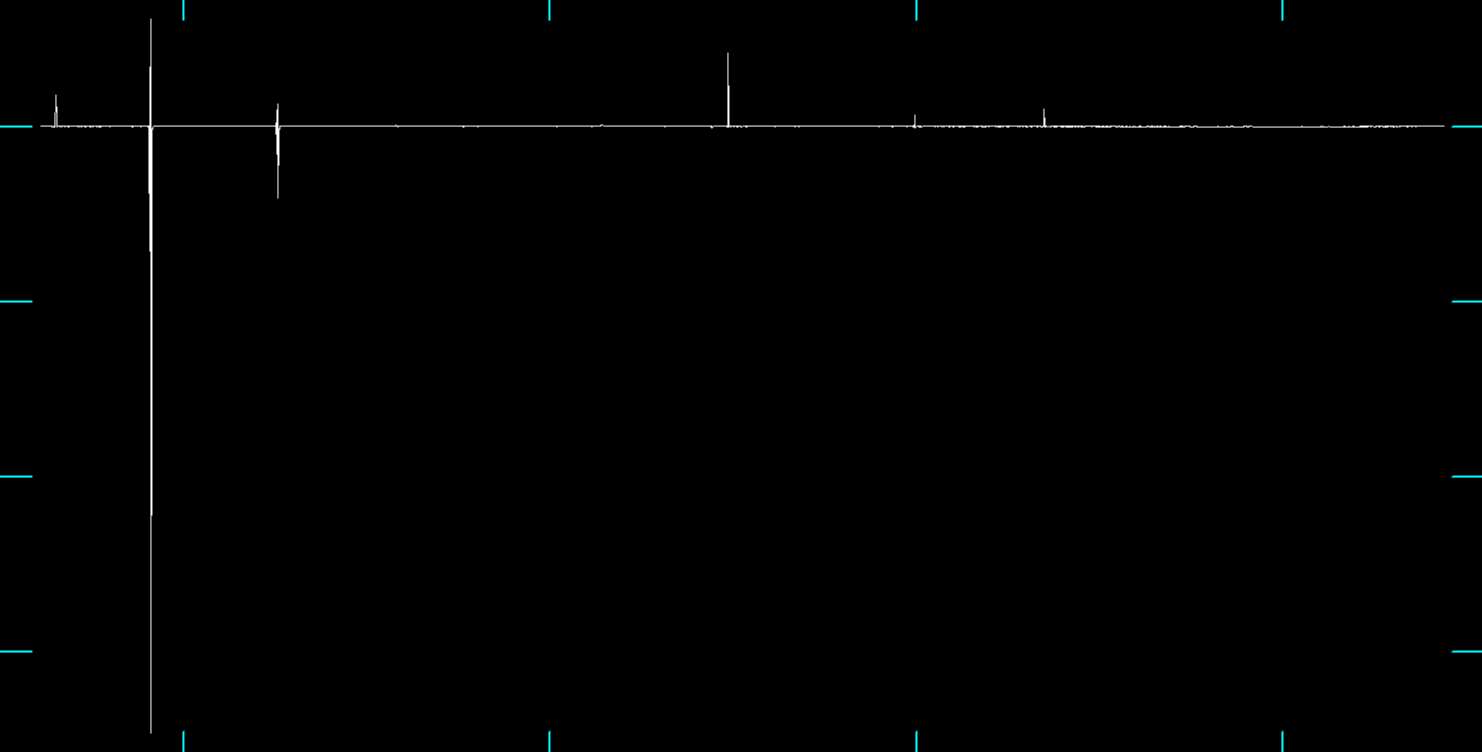
\includegraphics[width=\textwidth]{espectros/ex_corte.png}
        \caption{Exemplo de espectro bruto inteiro, com linhas maiores a serem removidas.}
    \end{subfigure}
    \begin{subfigure}[b]{0.65\textwidth}
        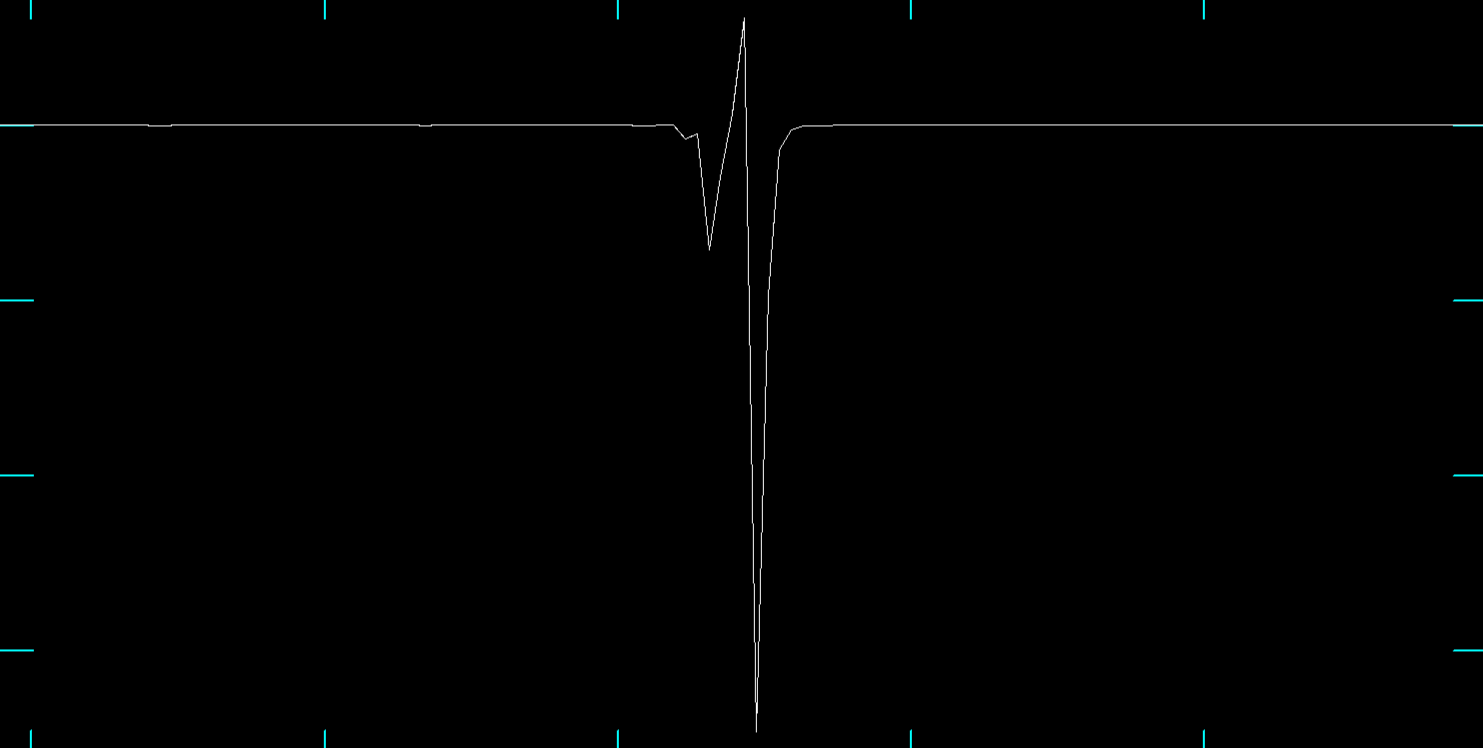
\includegraphics[width=\textwidth]{espectros/ex_corte_2.png}
        \caption{Exemplo de espectro bruto com ampliação em um exemplo de linha a ser removida.}
    \end{subfigure}
    \caption{Exemplos de espectros brutos obtidos no Gemini Sul, com linhas e picos a serem removidos para melhor visualização e análise.}
    \label{exemplo_remocao_linhas_ceu}
\end{figure}

Observamos a presença de linhas e picos no espectro que não estão associados a nenhuma emissão ou absorção conhecida. Esses picos apresentam uma amplitude significativamente maior do que o restante do espectro e necessitam ser eliminados. Geralmente, eles surgem após transições abruptas de subida e descida, ao contrário das emissões ou absorções genuínas, que tendem a ter uma aparência mais gaussiana.

Em cada um dos espectros, são eliminados os artefatos mais óbvios, resultando em espectros limpos e com uma escala de visualização que facilita a identificação de linhas de elementos.

Após processar todos os espectros dos objetos observados e realizar a limpeza necessária, procedemos à análise das possíveis linhas de emissão ou absorção. A primeira característica examinada para confirmar o tipo de objeto através do espectro é o redshift. A detecção de redshifts extremamente baixos é indicativa da proximidade do objeto dentro da Via Láctea. Vamos considerar como galáxias apenas objetos com $z > 0.002$, já que objetos com redshifts menores são geralmente estrelas da Via Láctea.

A observação de linhas de absorção no espectro acrescenta outro indicador significativo. Essas linhas resultam da absorção de luz pelas camadas exteriores da atmosfera estelar. Porém, vale ressaltar que a presença de linhas de absorção não é suficiente para confirmar a natureza estelar do objeto, pois as galáxias também podem apresentar esse tipo de linha.

Além disso, a detecção de linhas de emissão indica a presença de gás ionizado no objeto. Tais linhas estão comumente associadas a processos de formação estelar recente, em que regiões de gás interestelar são ionizadas por estrelas jovens e quentes, ou à atividade nuclear, onde são formadas em discos de acreção em torno de buracos negros supermassivos situados no centro das galáxias.

Para a análise das linhas, podemos usar como base alguns espectros de diferentes objetos observados pelo Sloan Digital Sky Survey (SDSS). Na Figura \ref{sdds_espectro}, mostramos alguns exemplos de espectros de alguns tipos de galáxias vindos do SDSS.

\begin{figure}[!ht]
    \begin{center}
    % \setcaptionmargin{1cm}
    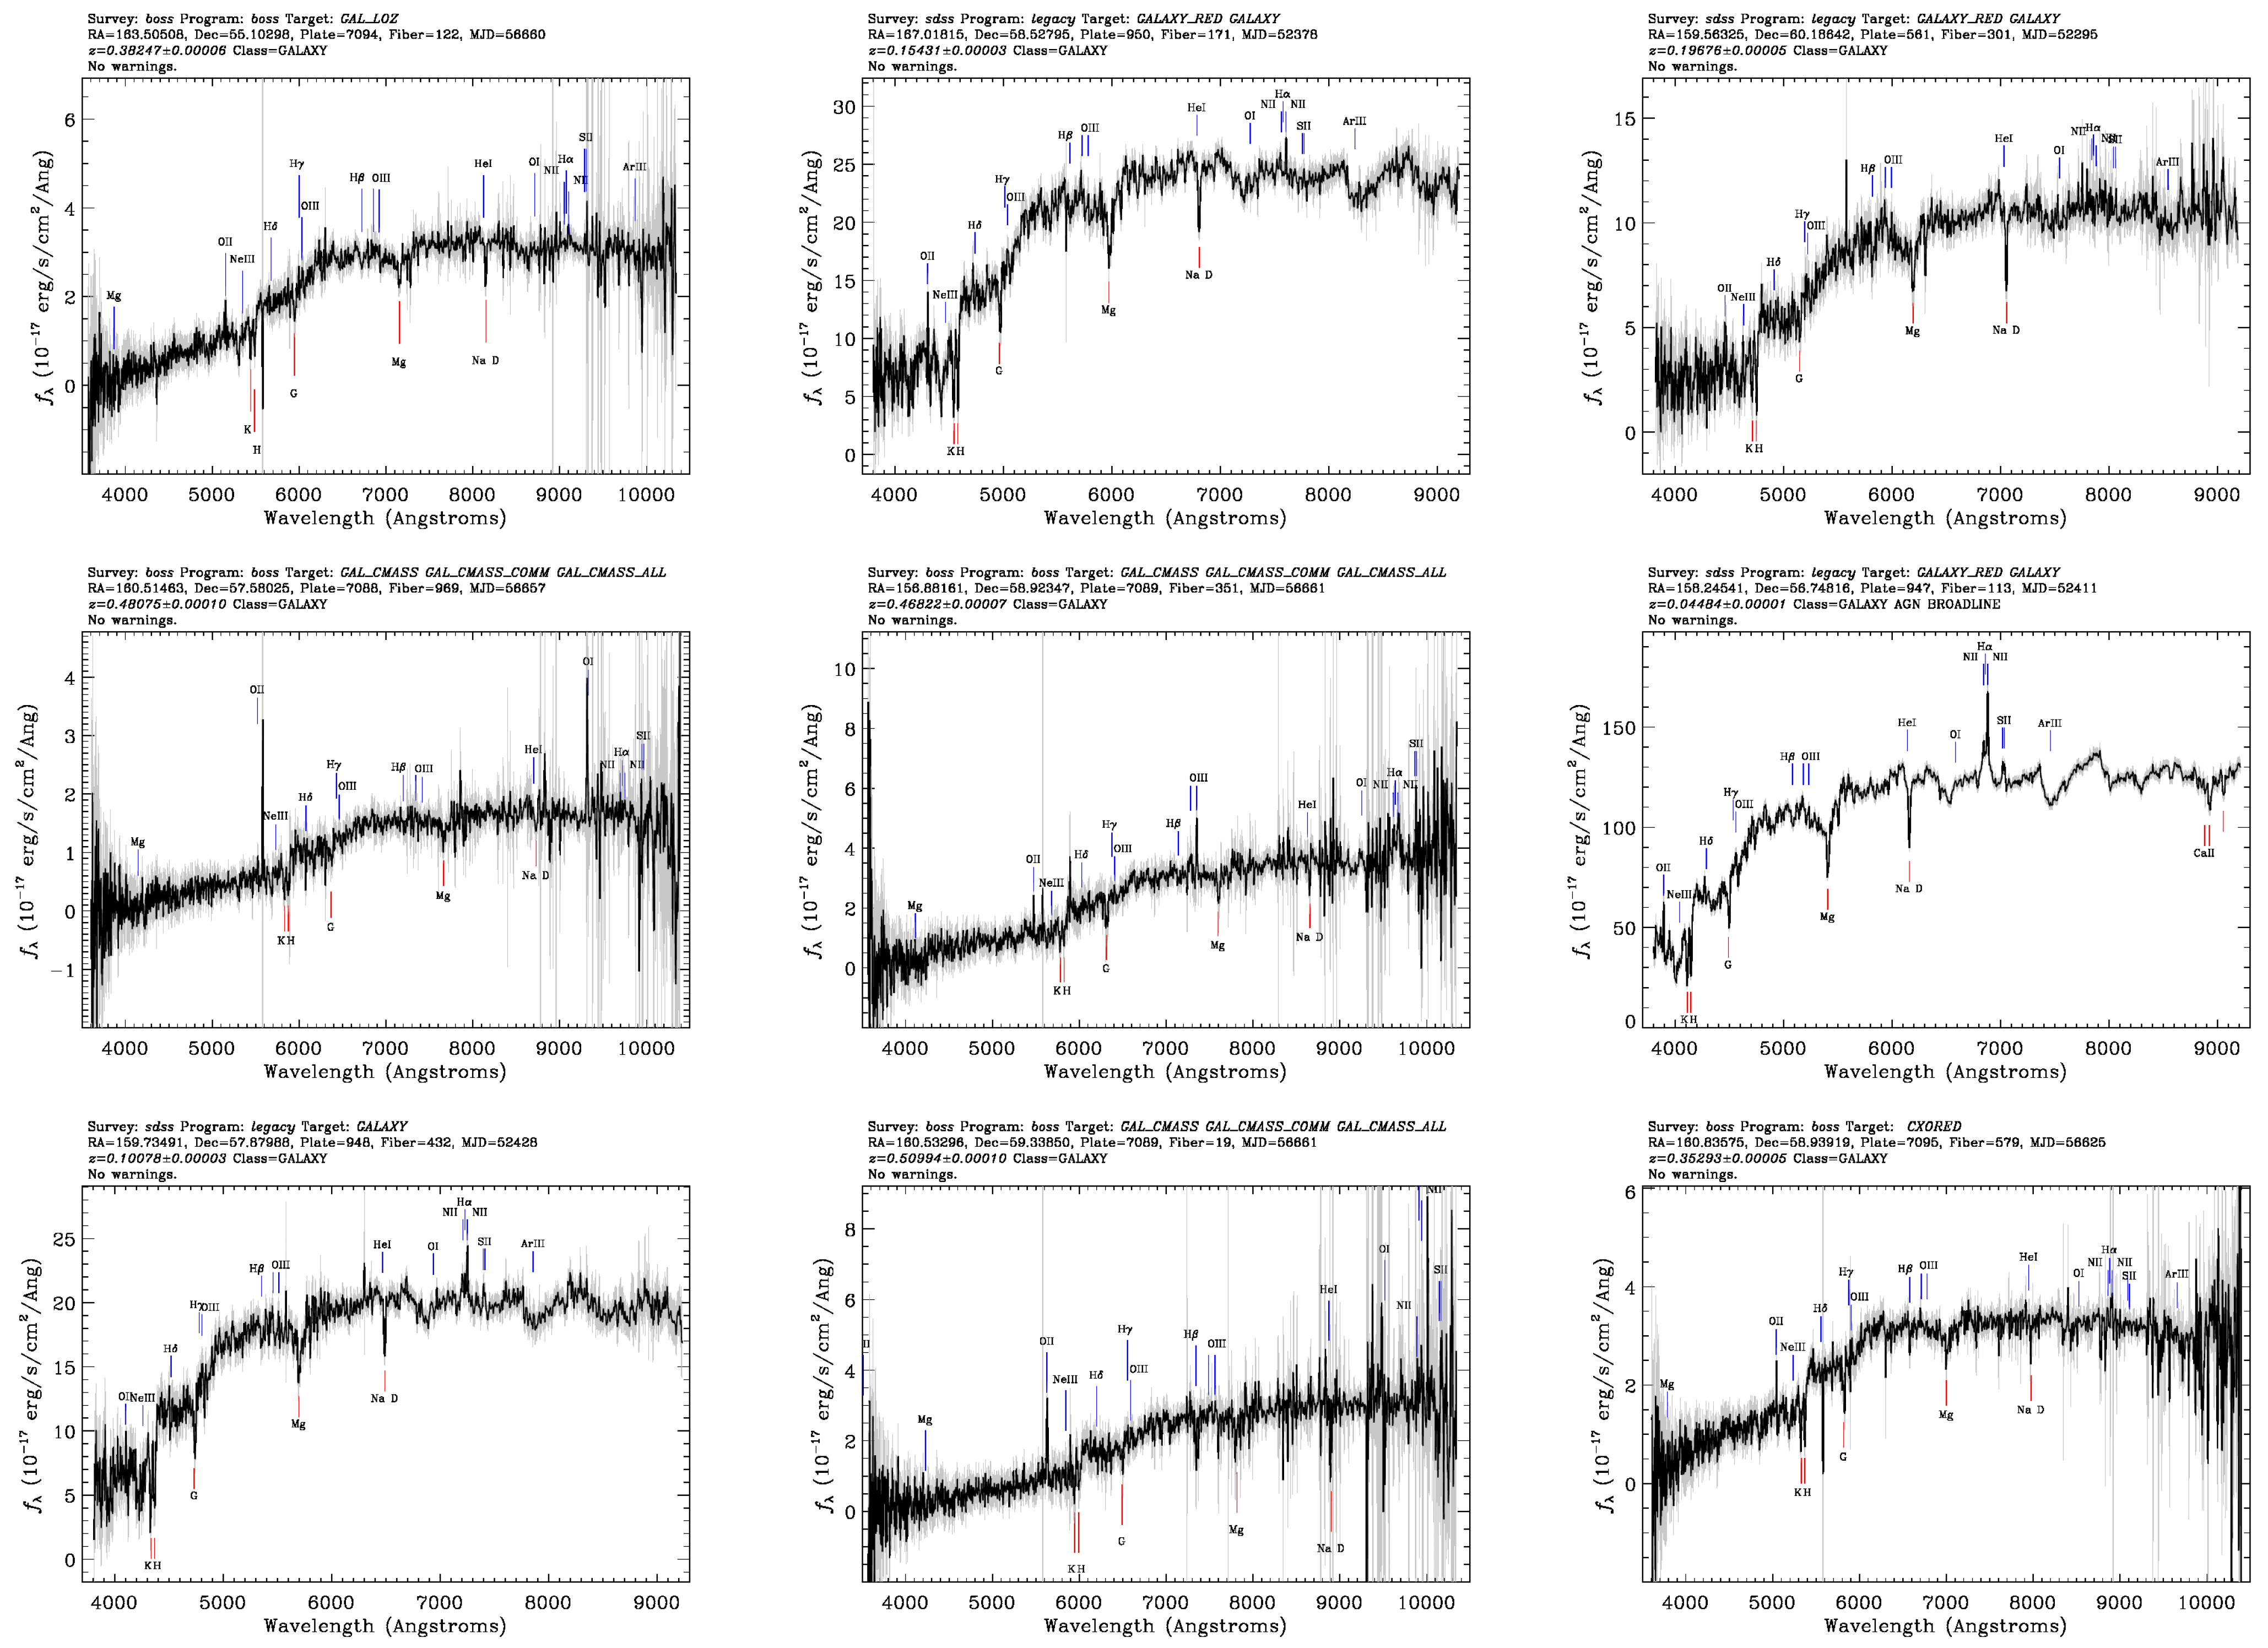
\includegraphics[width=1\columnwidth,angle=0]{espectros/sdds_espectro_01.png}
    \caption[]{Espectros de exemplo do SDSS de diferentes classes de objetos.}
    \label{sdds_espectro}
    \end{center}
\end{figure}    

Com base em espectros conhecidos e em tabelas das principais linhas de emissão e absorção (ex: $H\alpha$, $H\beta$, $[OIII]$, etc.), podemos procurar nos nossos espectros quais delas estão presentes e o quão deslocadas estão do esperado no repouso.

Nas próximas subseções, iremos mostrar os resultados das análises dos espectros para cada pedido de tempo de observação que foram descritos na seção \ref{sec:candidatas_espectroscopia}.

\section{Resultados espectros das candidatas}\label{sec:analise_espectros}
\subsection{Candidatas para espectroscopia}\label{sec:candidatas_espectroscopia}
Nesta seção, discutiremos os objetos selecionados para espectroscopia ao longo do projeto. Dando sequência a um projeto anterior de iniciação científica, foram selecionadas 18 candidatas a UCDs. Na época do projeto, foi submetido um pedido de tempo ao telescópio Gemini Sul para observação espectroscópica com o GMOS. Até o momento, 14 dessas candidatas foram observadas. Como parte do início deste projeto, foi feita a aquisição desses objetos para análise dos espectros.

Na Tabela \ref{candidatas_espectroscopia_1}, temos a lista dessas candidatas observadas, com suas respectivas coordenadas. Utilizando o Legacy Survey Sky Browser\footnote{Legacy Survey Sky Browser}, apresentamos na Figura \ref{candidatas_espectroscopia_1_img} as imagens desses objetos.

\begin{table}[!ht]
    \centering
    \caption{Conjunto de candidatas a UCDs observadas com o GMOS no telescópio Gemini Sul, selecionadas de um projeto anterior. A coluna $OBJ_{name}$ é o nome interno da candidata utilizado no pedido de tempo do Gemini.} 
    \begin{tabular}{lcc}
        \toprule
        $OBJ_{name}$ & RA     & DEC     \\
        \midrule
        UCG01     & 47,708 & -34,157 \\
        UCG02     & 47,960 & -33,174 \\
        UCG03     & 49,910 & -31,523 \\
        UCG04     & 53,753 & -37,155 \\
        UCG05     & 53,820 & -35,837 \\
        UCG06     & 54,115 & -36,845 \\
        UCG07     & 54,214 & -36,814 \\
        UCG08     & 54,912 & -35,439 \\
        UCG09     & 55,010 & -35,535 \\
        UCG10     & 55,056 & -37,895 \\
        UCG11     & 55,211 & -38,048 \\
        UCG12     & 55,315 & -37,020 \\
        UCG13     & 55,333 & -36,653 \\
        UCG14     & 55,673 & -36,541 \\
        UCG15     & 57,272 & -35,515 \\
        UCG16     & 57,468 & -34,663 \\
        UCG17     & 58,035 & -37,111 \\
        UCG18     & 58,083 & -36,298 \\
        \bottomrule
    \end{tabular}
    \label{candidatas_espectroscopia_1}
\end{table}


\begin{figure}[!ht]
    \centering
    \captionsetup{justification=centering}
    \begin{subfigure}[b]{0.22\textwidth}
        \includegraphics[width=\textwidth]{proposatal_candidatas_1/UCG01.png}
        \caption{UCG01}
    \end{subfigure}
    \begin{subfigure}[b]{0.22\textwidth}
        \includegraphics[width=\textwidth]{proposatal_candidatas_1/UCG02.png}
        \caption{UCG02}
    \end{subfigure}
    \begin{subfigure}[b]{0.22\textwidth}
        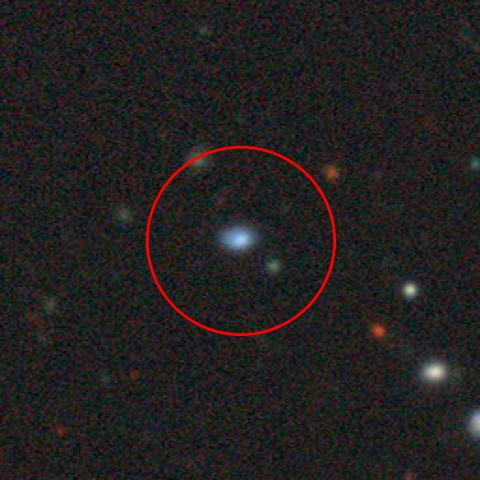
\includegraphics[width=\textwidth]{proposatal_candidatas_1/UCG03.jpg}
        \caption{UCG03}
    \end{subfigure}
    \begin{subfigure}[b]{0.22\textwidth}
        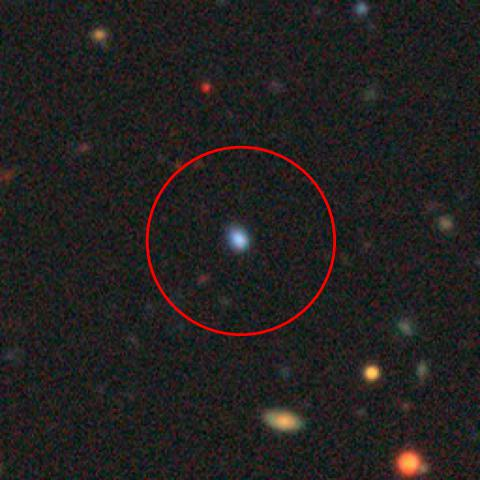
\includegraphics[width=\textwidth]{proposatal_candidatas_1/UCG04.jpg}
        \caption{UCG04}
    \end{subfigure}
    \begin{subfigure}[b]{0.22\textwidth}
        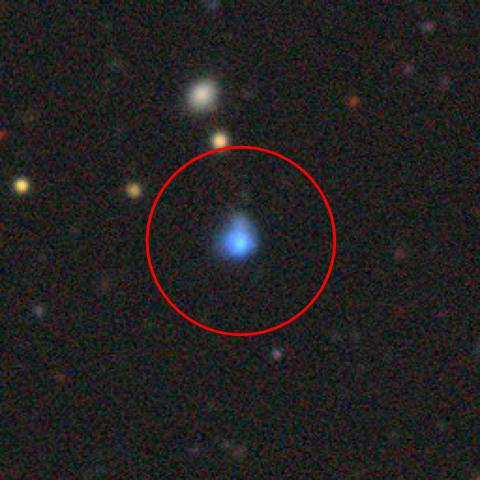
\includegraphics[width=\textwidth]{proposatal_candidatas_1/UCG05.jpg}
        \caption{UCG05}
    \end{subfigure}
    \begin{subfigure}[b]{0.22\textwidth}
        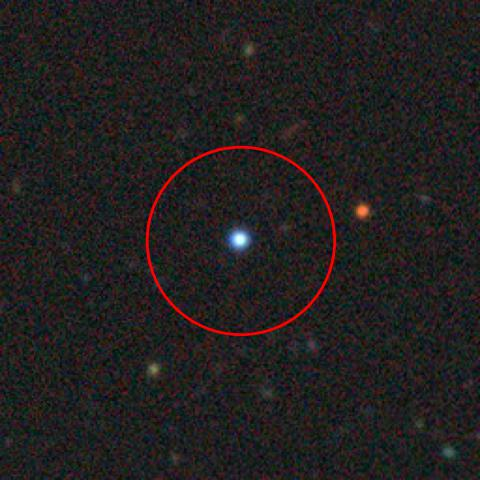
\includegraphics[width=\textwidth]{proposatal_candidatas_1/UCG06.jpg}
        \caption{UCG06}
    \end{subfigure}
    \begin{subfigure}[b]{0.22\textwidth}
        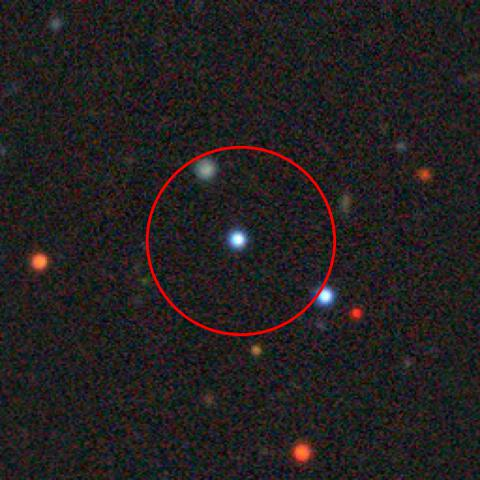
\includegraphics[width=\textwidth]{proposatal_candidatas_1/UCG07.jpg}
        \caption{UCG07}
    \end{subfigure}
    \begin{subfigure}[b]{0.22\textwidth}
        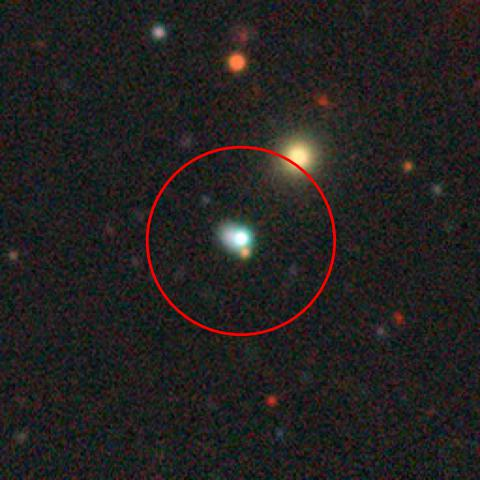
\includegraphics[width=\textwidth]{proposatal_candidatas_1/UCG08.jpg}
        \caption{UCG08}
    \end{subfigure}
    \begin{subfigure}[b]{0.22\textwidth}
        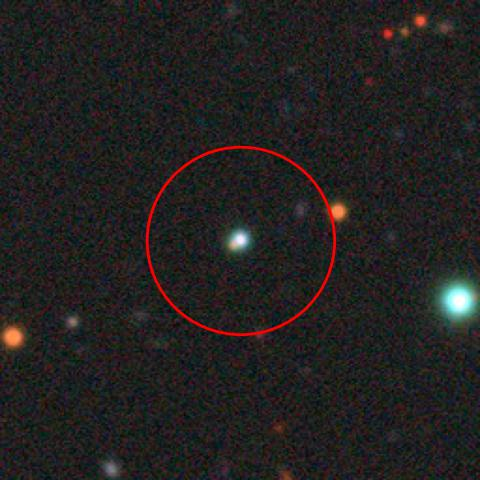
\includegraphics[width=\textwidth]{proposatal_candidatas_1/UCG09.jpg}
        \caption{UCG09}
    \end{subfigure}
    \begin{subfigure}[b]{0.22\textwidth}
        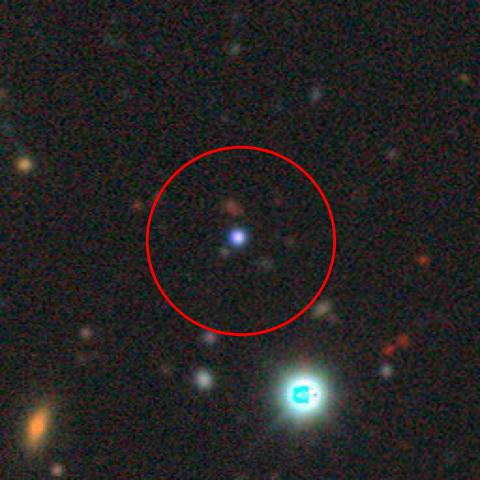
\includegraphics[width=\textwidth]{proposatal_candidatas_1/UCG10.jpg}
        \caption{UCG10}
    \end{subfigure}
    \begin{subfigure}[b]{0.22\textwidth}
        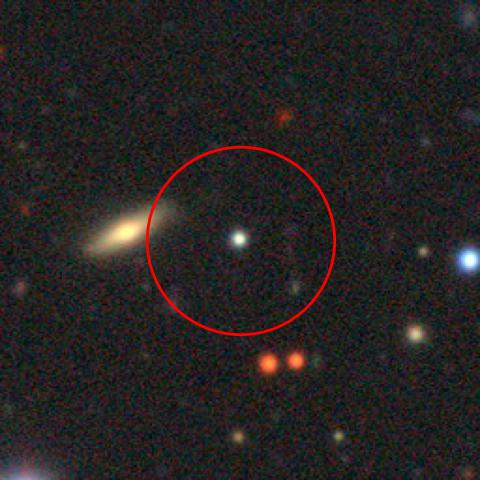
\includegraphics[width=\textwidth]{proposatal_candidatas_1/UCG11.jpg}
        \caption{UCG11}
    \end{subfigure}
    \begin{subfigure}[b]{0.22\textwidth}
        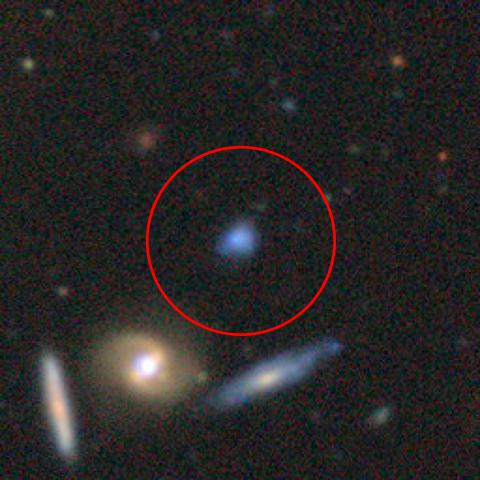
\includegraphics[width=\textwidth]{proposatal_candidatas_1/UCG12.jpg}
        \caption{UCG12}
    \end{subfigure}
    \begin{subfigure}[b]{0.22\textwidth}
        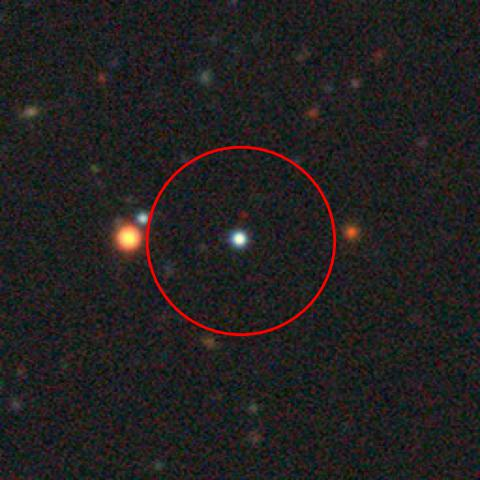
\includegraphics[width=\textwidth]{proposatal_candidatas_1/UCG13.jpg}
        \caption{UCG13}
    \end{subfigure}
    \begin{subfigure}[b]{0.22\textwidth}
        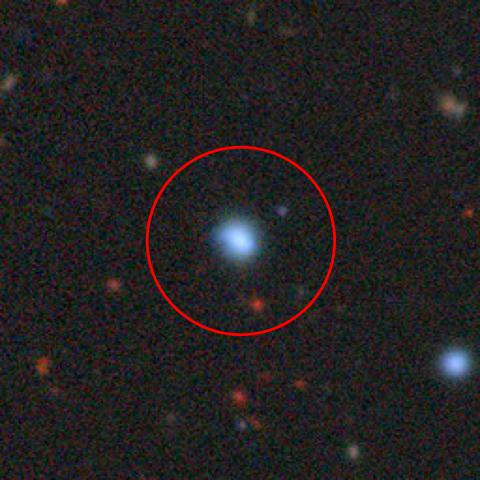
\includegraphics[width=\textwidth]{proposatal_candidatas_1/UCG14.jpg}
        \caption{UCG14}
    \end{subfigure}
    \begin{subfigure}[b]{0.22\textwidth}
        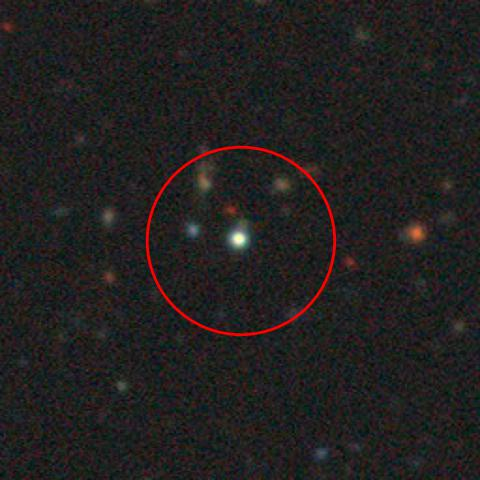
\includegraphics[width=\textwidth]{proposatal_candidatas_1/UCG15.jpg}
        \caption{UCG15}
    \end{subfigure}
    \begin{subfigure}[b]{0.22\textwidth}
        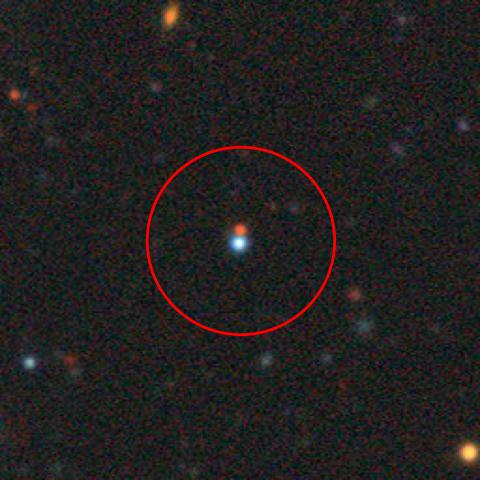
\includegraphics[width=\textwidth]{proposatal_candidatas_1/UCG16.jpg}
        \caption{UCG16}
    \end{subfigure}
    \begin{subfigure}[b]{0.22\textwidth}
        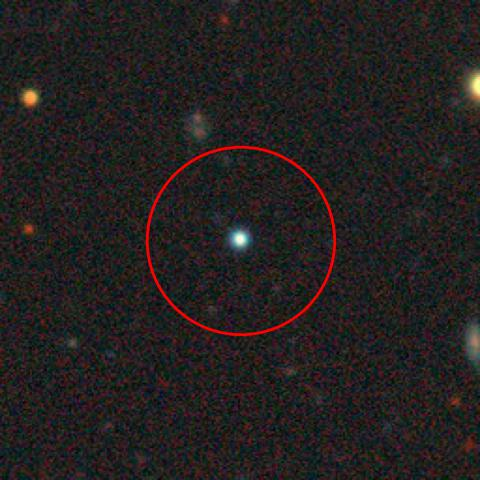
\includegraphics[width=\textwidth]{proposatal_candidatas_1/UCG17.jpg}
        \caption{UCG17}
    \end{subfigure}
    \begin{subfigure}[b]{0.22\textwidth}
        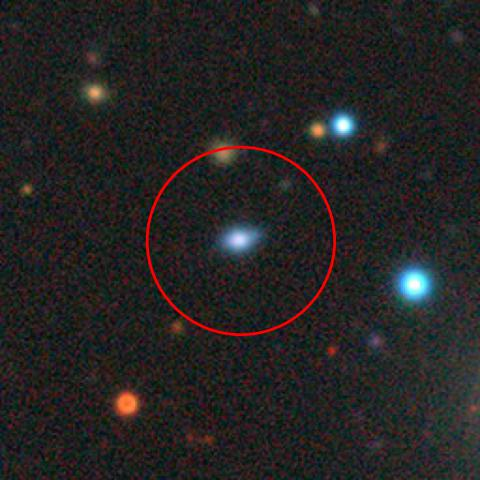
\includegraphics[width=\textwidth]{proposatal_candidatas_1/UCG18.jpg}
        \caption{UCG18}
    \end{subfigure}
    \caption{Imagens das candidatas a UCDs observadas com o GMOS no telescópio Gemini Sul, selecionadas de um projeto anterior. Imagens obtidas pelo Legacy Survey. Os nomes correspondem ao mesmo nome do objeto da Tabela \ref{candidatas_espectroscopia_1}.}
    \label{candidatas_espectroscopia_1_img}
\end{figure}

\subsection{Resultado espectros pedidos de tempo}\label{subsection:resultado_espectros_candidatas}

Nesta seção, comentaremos sobre os resultados obtidos das candidatas descritas na seção \ref{sec:candidatas_espectroscopia}. Para o primeiro pedido de tempo, tivemos 14 objetos analisados. Os espectros desses objetos, depois de limparmos os artefatos e ruídos para análise, são apresentados no conjunto das Figuras \ref{espectros_candidatas_1_p1} e \ref{espectros_candidatas_1_p2}.

\begin{figure}[!ht]
    \centering
    \captionsetup{justification=centering}
    \begin{subfigure}[b]{0.45\textwidth}
        \includegraphics[width=\textwidth]{espectros/UCG01.png}
        \caption{UCG01}
    \end{subfigure}
    \begin{subfigure}[b]{0.45\textwidth}
        \includegraphics[width=\textwidth]{espectros/UCG02.png}
        \caption{UCG02}
    \end{subfigure}
    \begin{subfigure}[b]{0.45\textwidth}
        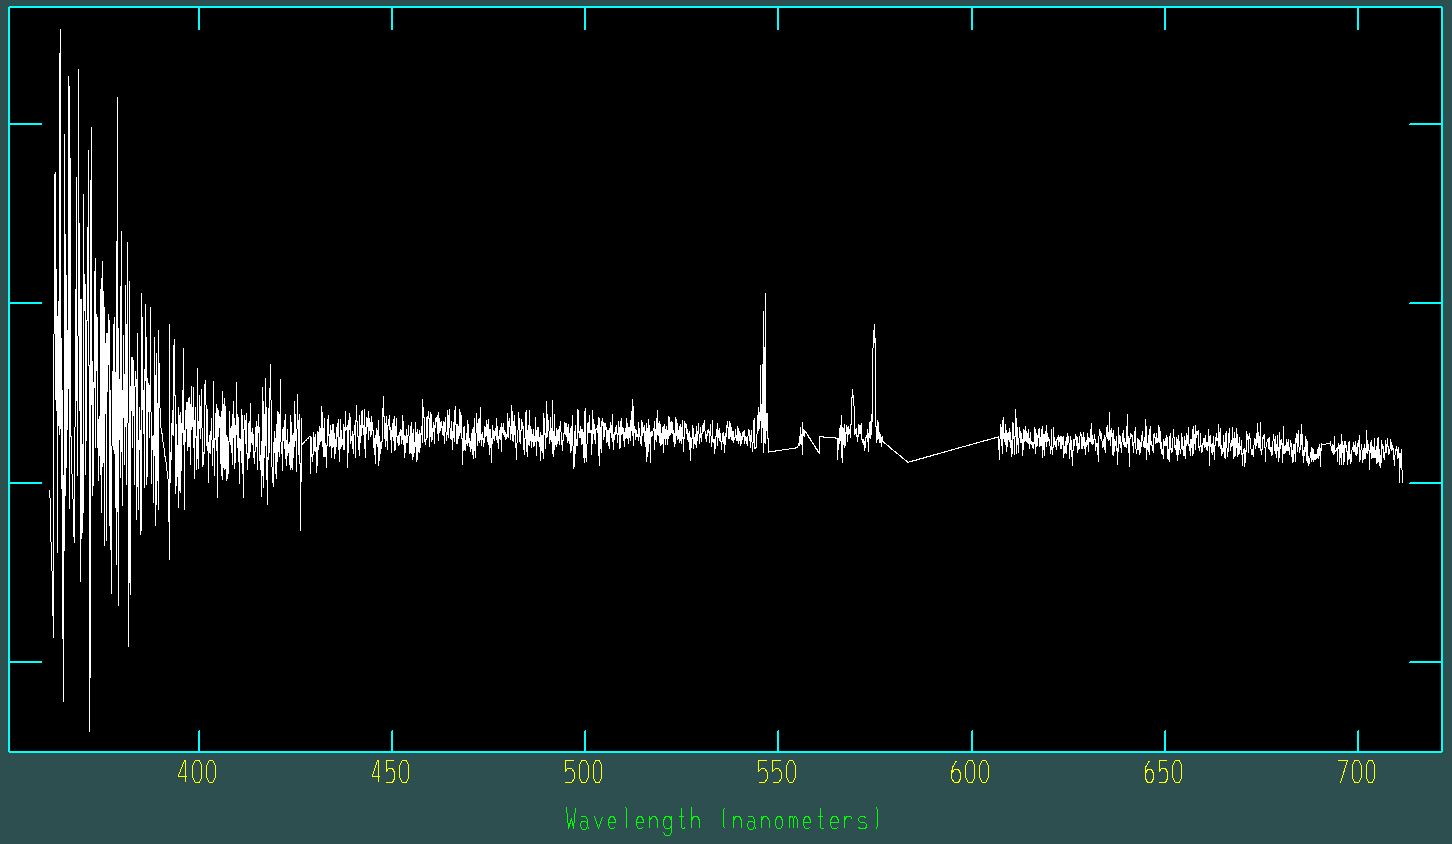
\includegraphics[width=\textwidth]{espectros/UCG03.png}
        \caption{UCG01}
    \end{subfigure}
    \begin{subfigure}[b]{0.45\textwidth}
        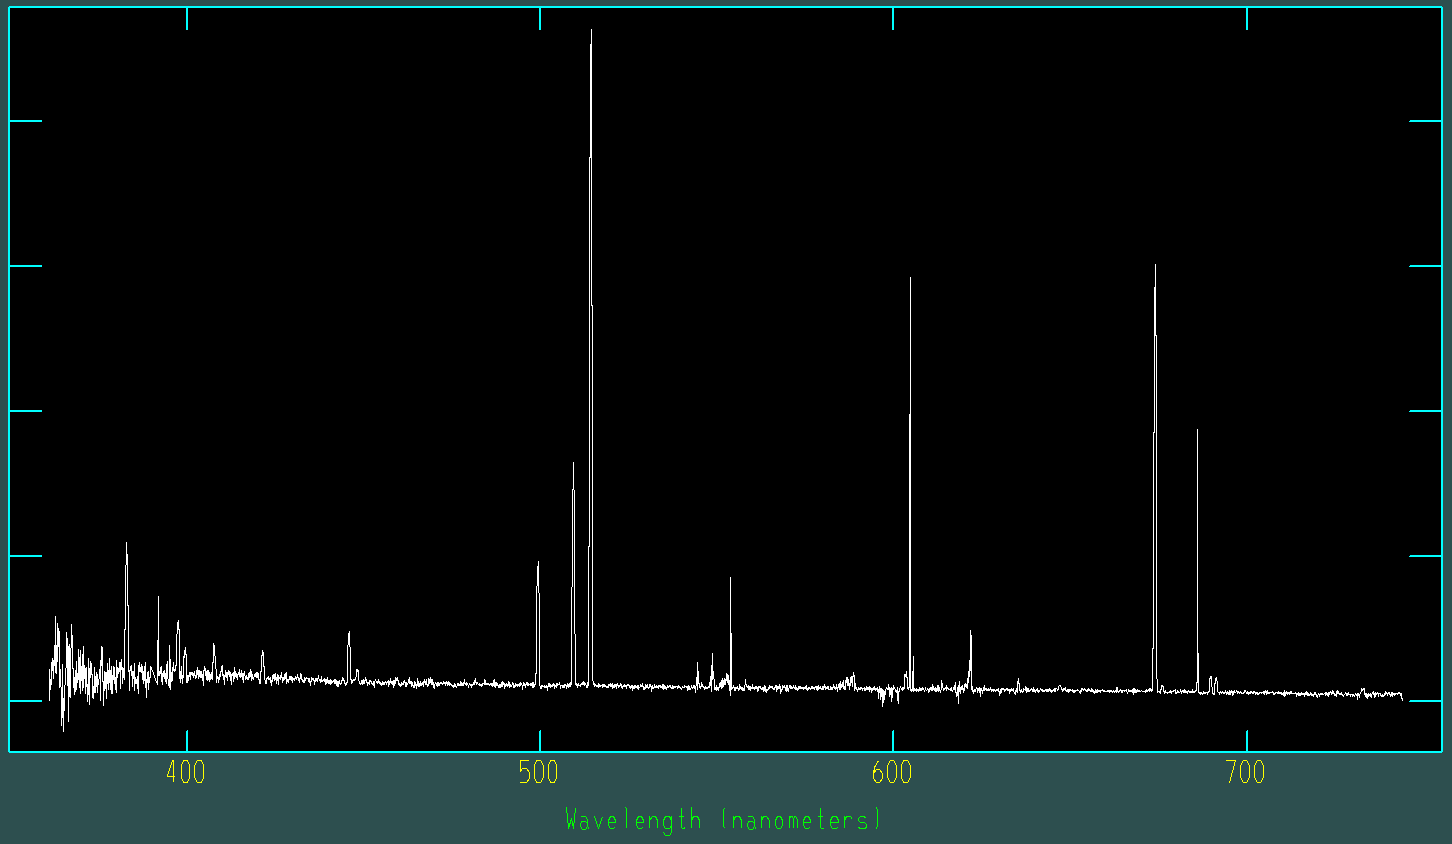
\includegraphics[width=\textwidth]{espectros/UCG05.png}
        \caption{UCG01}
    \end{subfigure}
    \begin{subfigure}[b]{0.45\textwidth}
        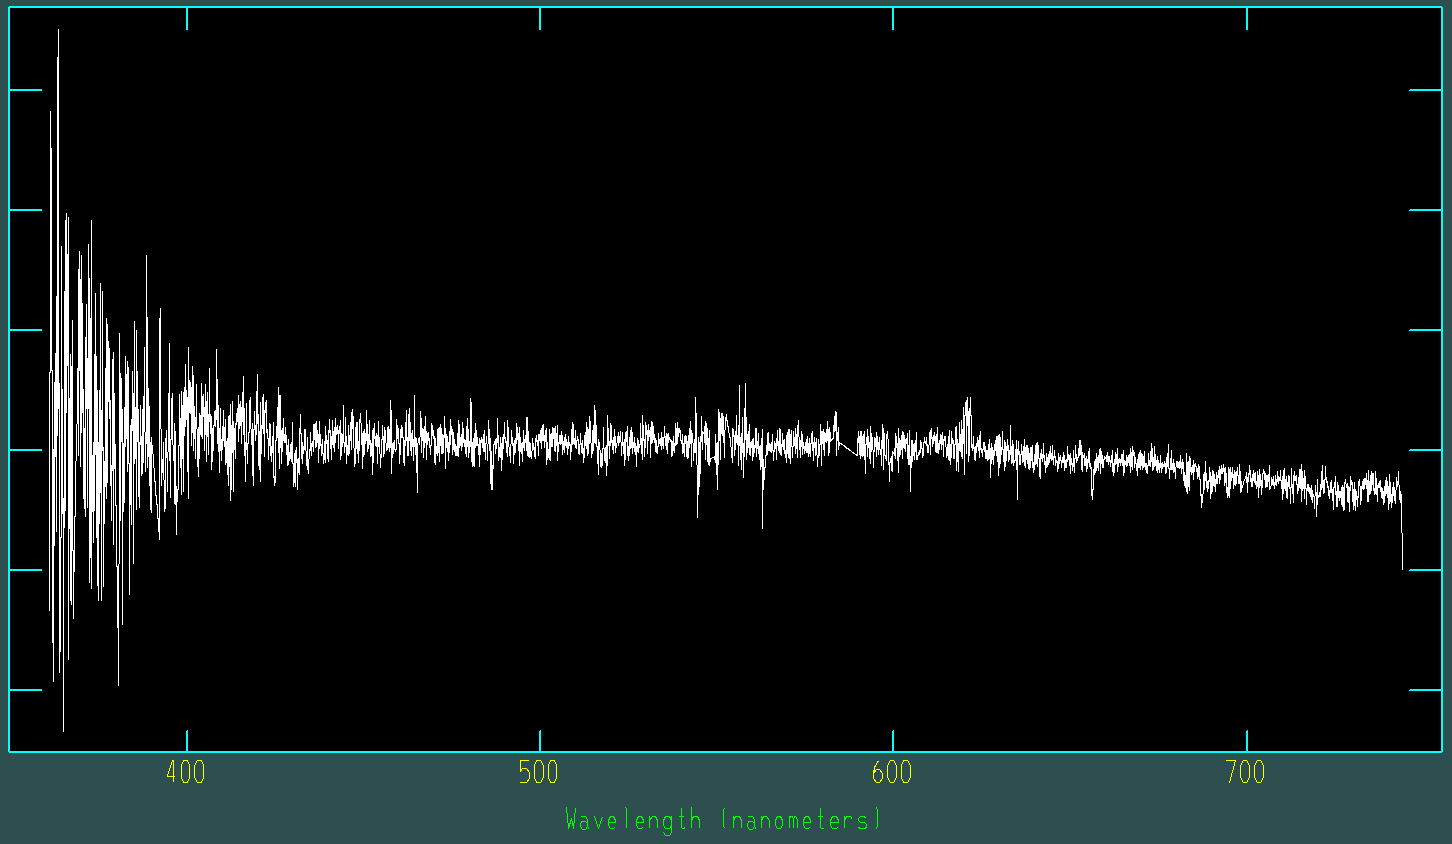
\includegraphics[width=\textwidth]{espectros/UCG06.png}
        \caption{UCG01}
    \end{subfigure}
    \begin{subfigure}[b]{0.45\textwidth}
        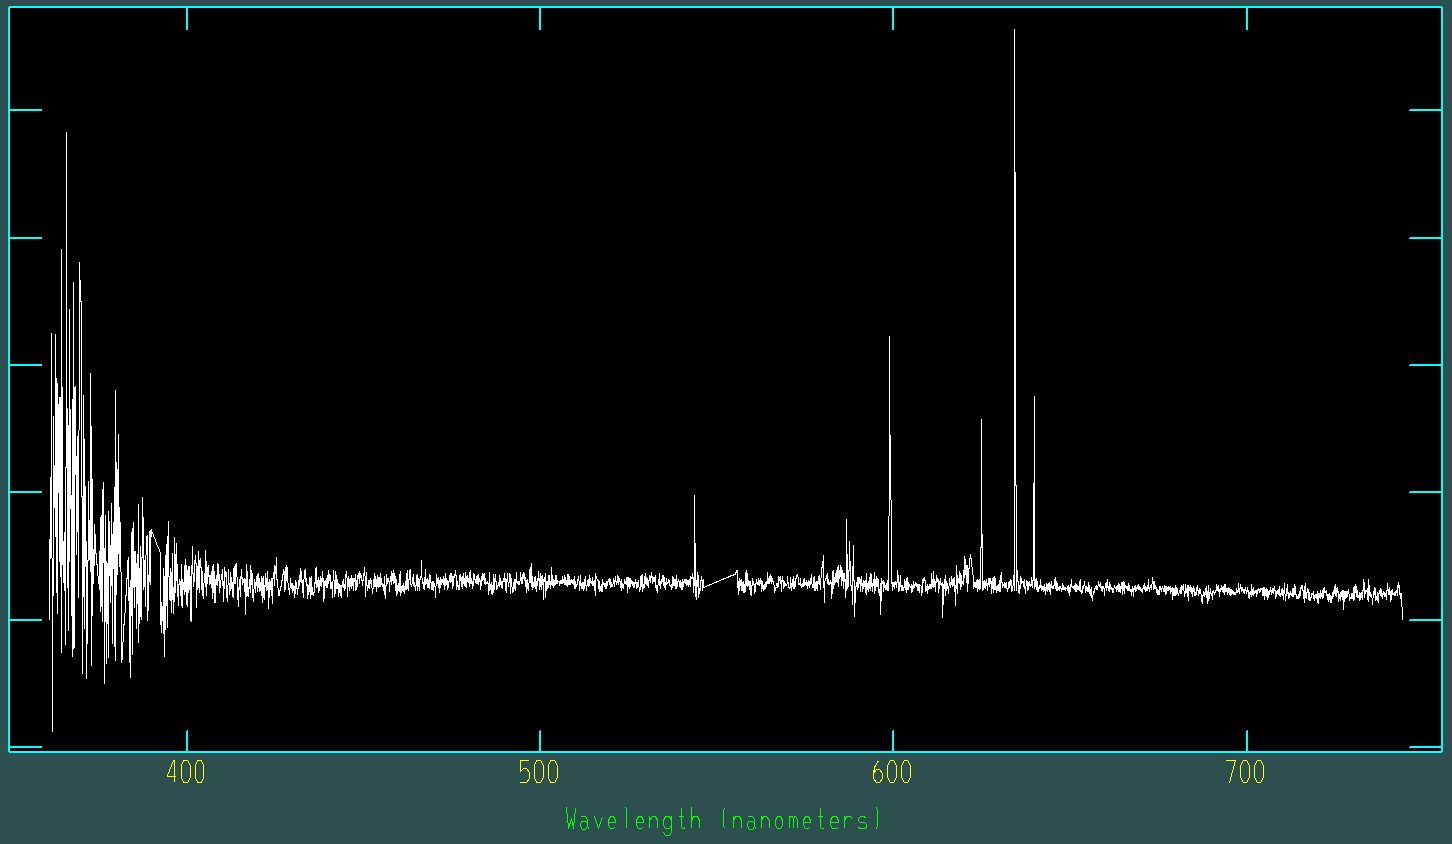
\includegraphics[width=\textwidth]{espectros/UCG07.png}
        \caption{UCG01}
    \end{subfigure}
    \begin{subfigure}[b]{0.45\textwidth}
        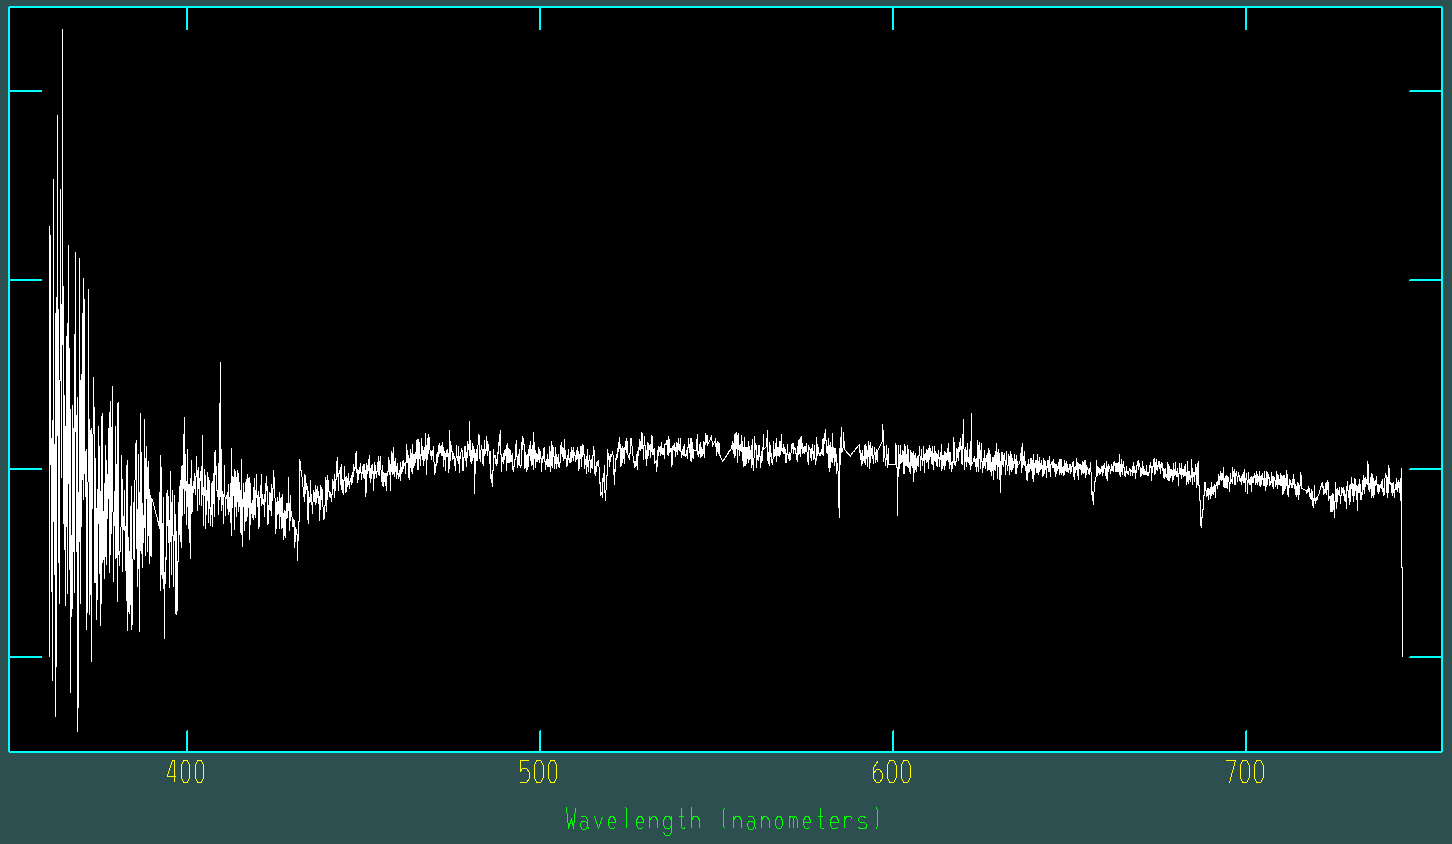
\includegraphics[width=\textwidth]{espectros/UCG08.png}
        \caption{UCG01}
    \end{subfigure}
    \begin{subfigure}[b]{0.45\textwidth}
        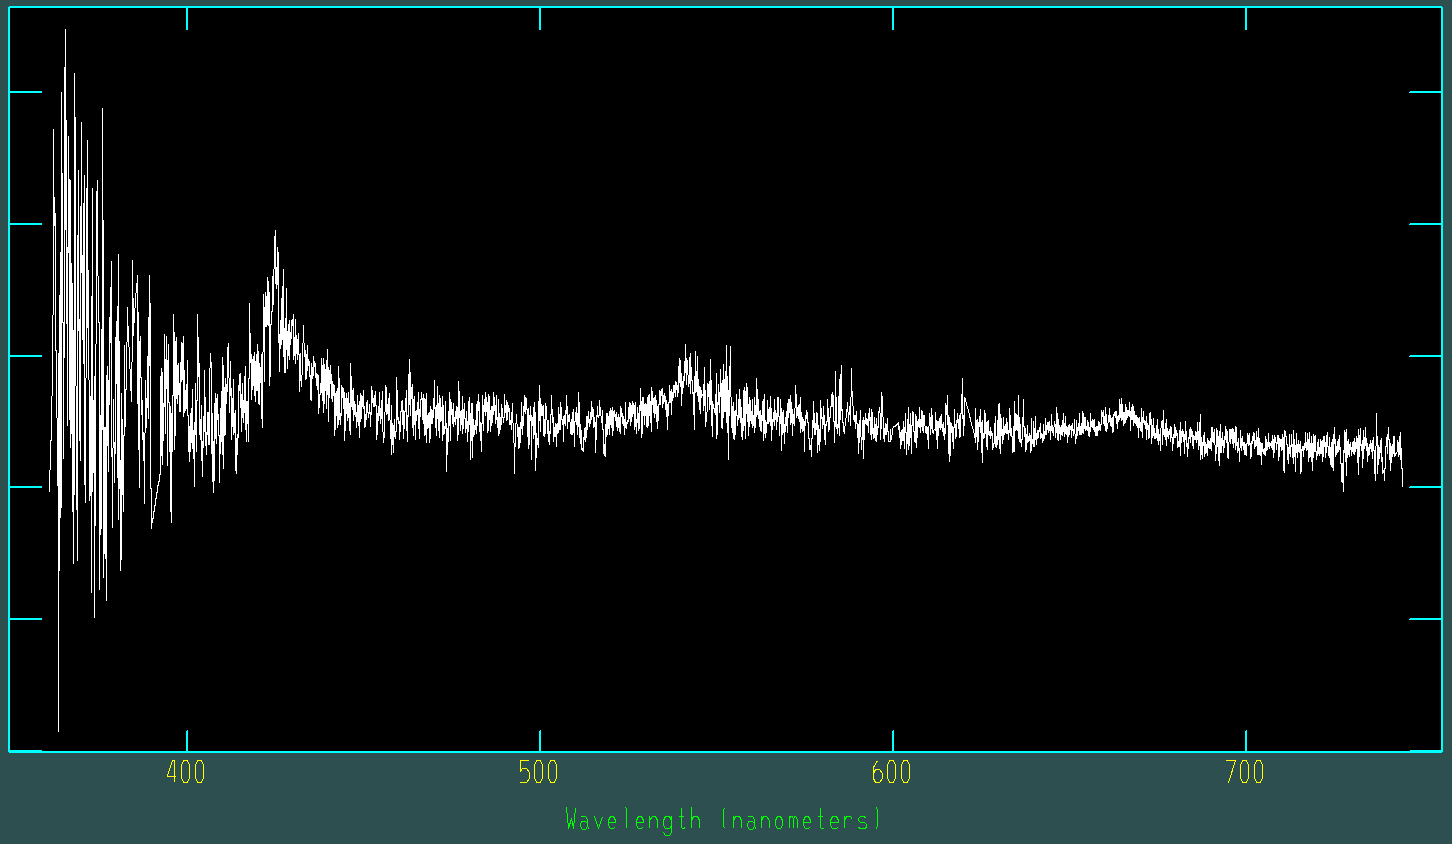
\includegraphics[width=\textwidth]{espectros/UCG10.png}
        \caption{UCG01}
    \end{subfigure}
    \caption{Espectros das candidatas a UCDs do primeiro pedido de tempo observadas no Gemini Sul. Os nomes \textit{UCG} correspondem ao nome interno usado para o pedido de tempo de observação. Os objetos com contagem faltando foram aqueles não observados por algum problema no pedido de tempo.}
    \label{espectros_candidatas_1_p1}
\end{figure}


\begin{figure}[!ht]
    \centering
    \begin{subfigure}[b]{0.45\textwidth}
        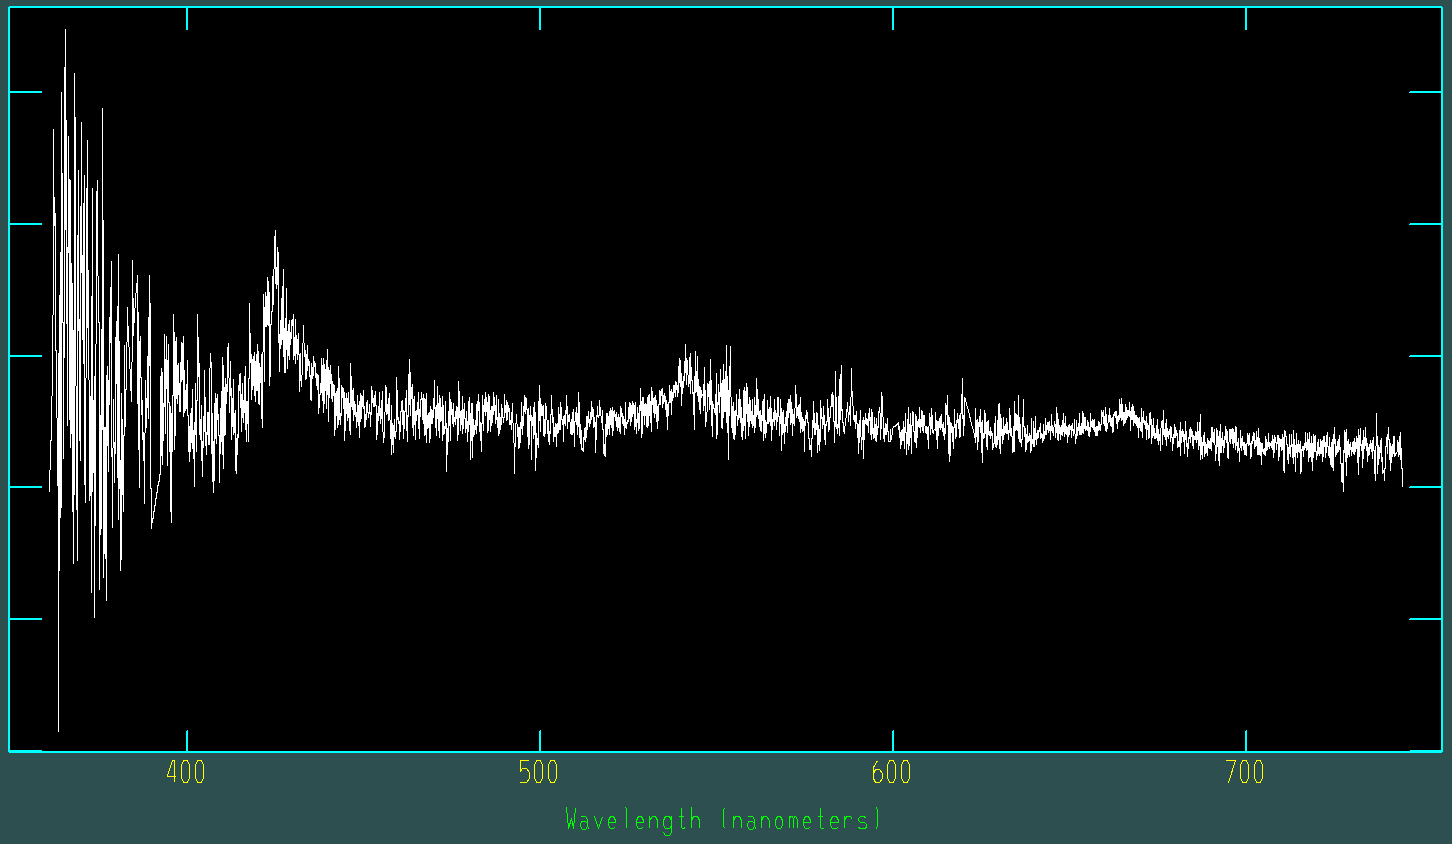
\includegraphics[width=\textwidth]{espectros/UCG10.png}
        \caption{UCG01}
    \end{subfigure}
    \begin{subfigure}[b]{0.45\textwidth}
        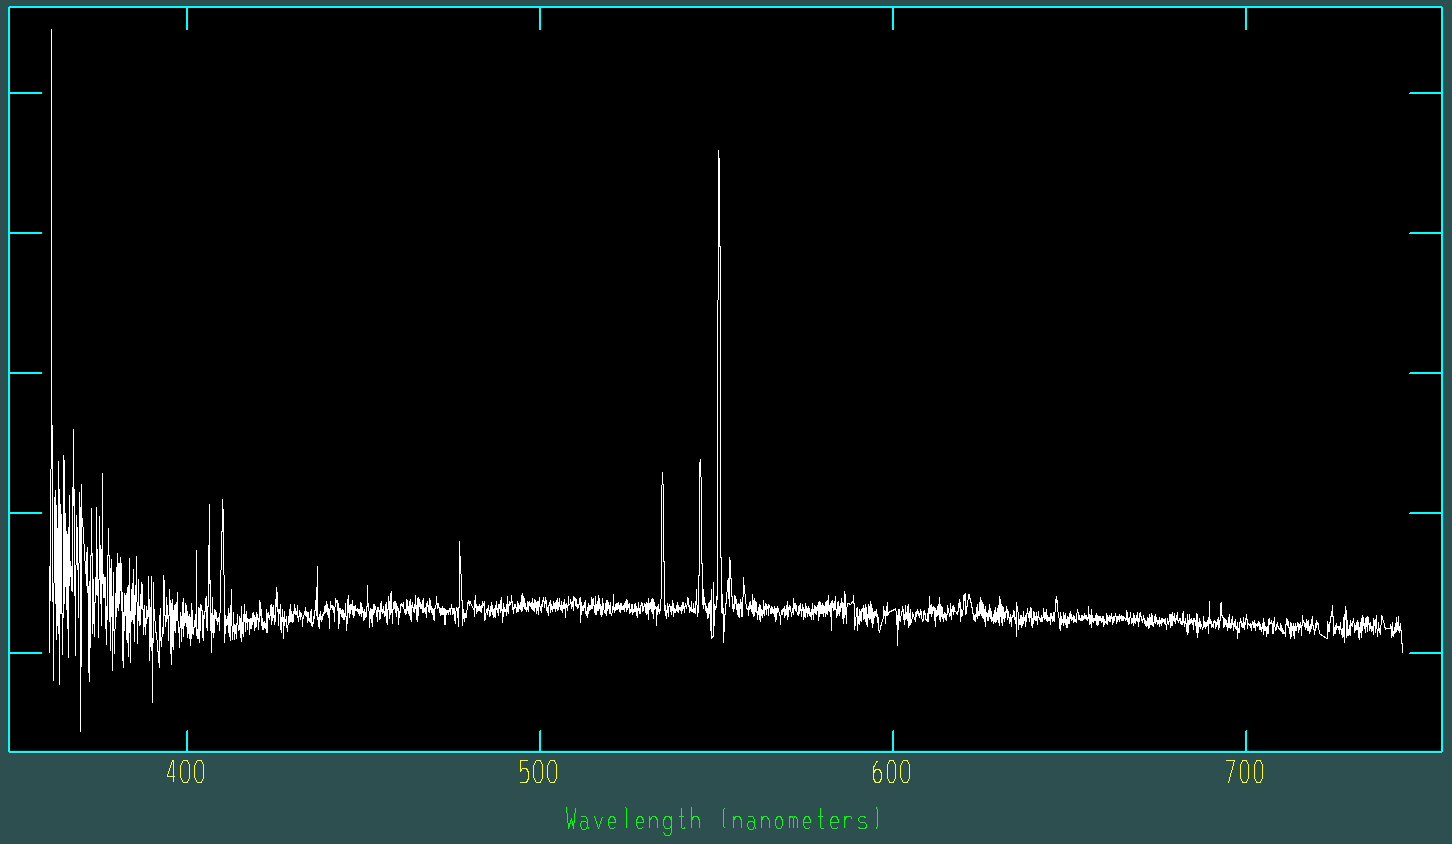
\includegraphics[width=\textwidth]{espectros/UCG12.png}
        \caption{UCG01}
    \end{subfigure}
    \begin{subfigure}[b]{0.45\textwidth}
        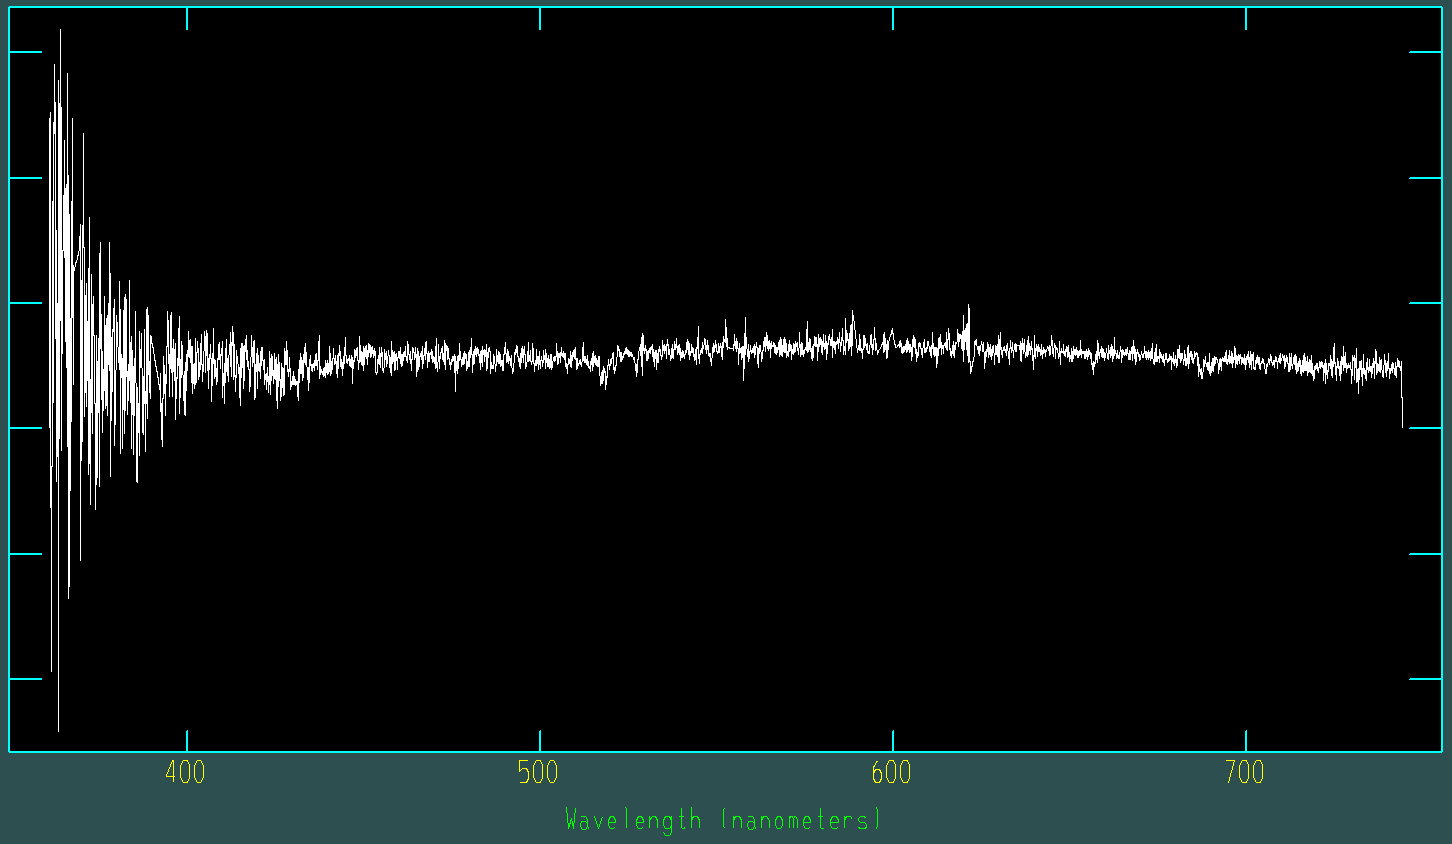
\includegraphics[width=\textwidth]{espectros/UCG13.png}
        \caption{UCG01}
    \end{subfigure}
    \begin{subfigure}[b]{0.45\textwidth}
        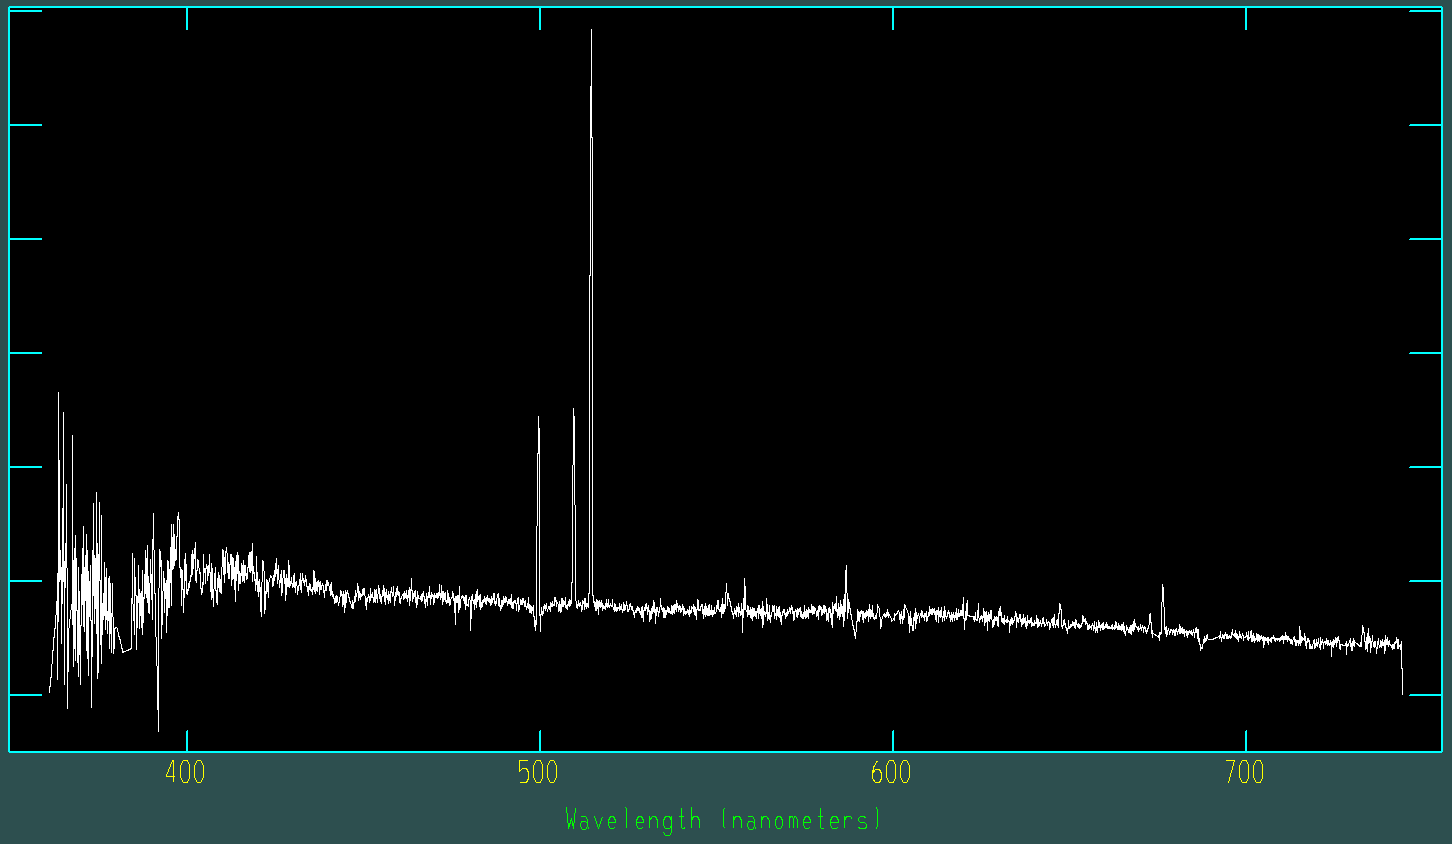
\includegraphics[width=\textwidth]{espectros/UCG14.png}
        \caption{UCG01}
    \end{subfigure}
    \begin{subfigure}[b]{0.45\textwidth}
        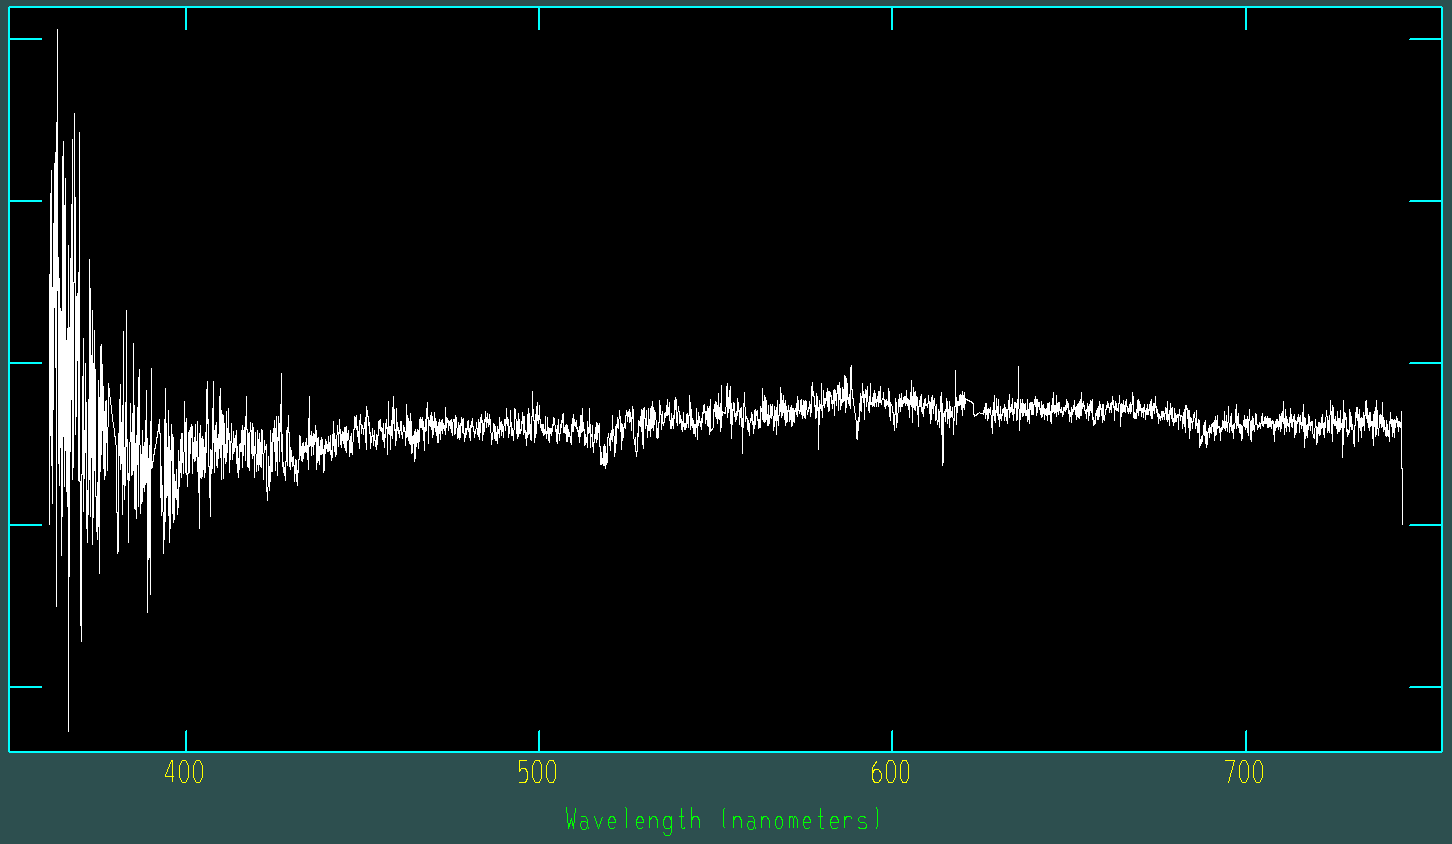
\includegraphics[width=\textwidth]{espectros/UCG15.png}
        \caption{UCG01}
    \end{subfigure}
    \begin{subfigure}[b]{0.45\textwidth}
        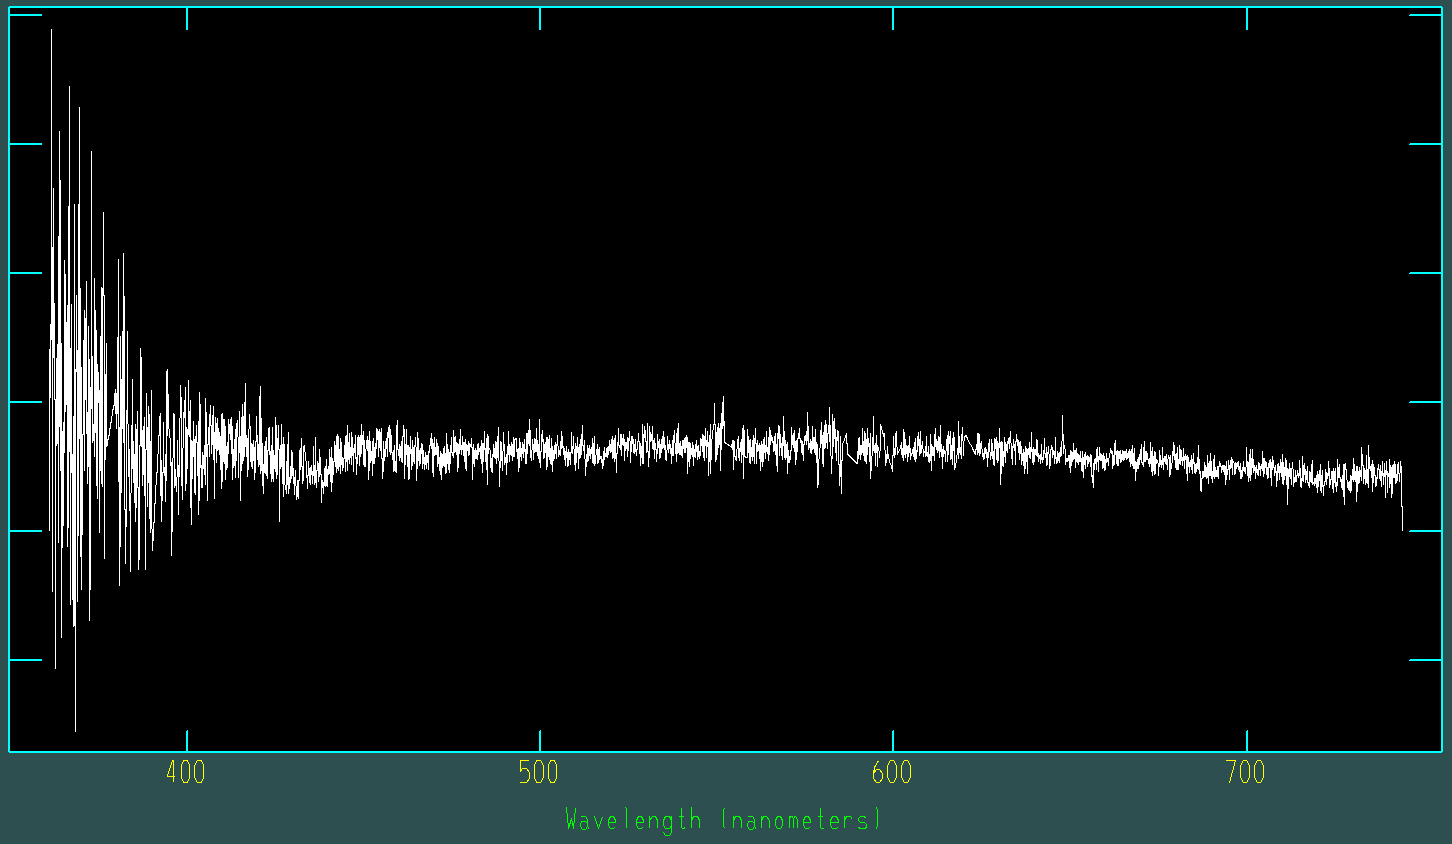
\includegraphics[width=\textwidth]{espectros/UCG16.png}
        \caption{UCG01}
    \end{subfigure}
    \begin{subfigure}[b]{0.45\textwidth}
        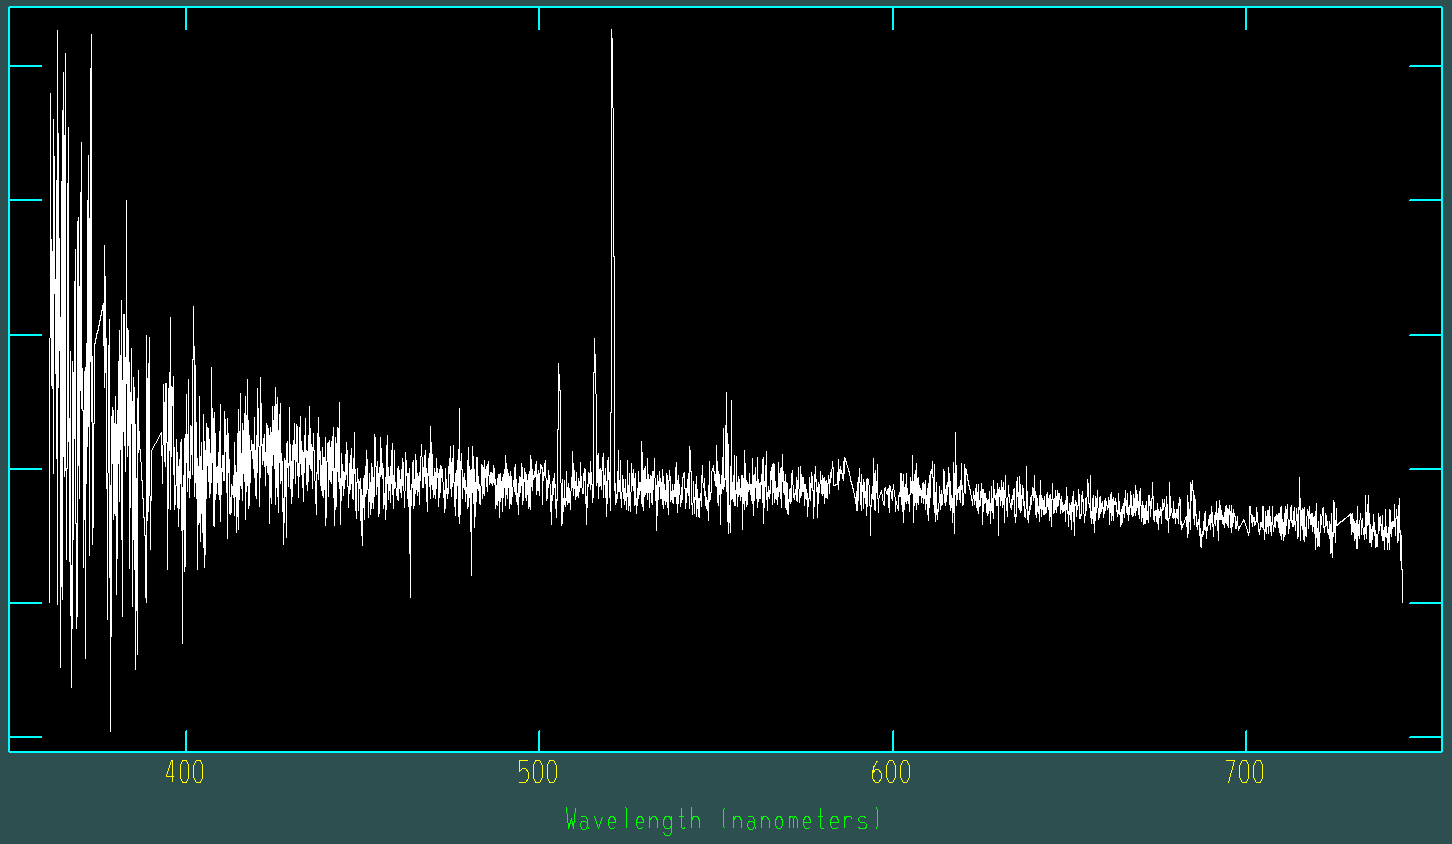
\includegraphics[width=\textwidth]{espectros/UCG18.png}
        \caption{UCG01}
    \end{subfigure}
    \caption{Espectros das candidatas a UCDs do primeiro pedido de tempo observadas no Gemini Sul. Os nomes \textit{UCG} correspondem ao nome interno usado para o pedido de tempo de observação. Os objetos com contagem faltando foram aqueles não observados por algum problema no pedido de tempo.}
    \label{espectros_candidatas_1_p2}
\end{figure}

A partir de cada espectro, para a confirmação do tipo do objeto e se ele faz parte do aglomerado, analisamos as linhas de emissão e absorção presentes. Na Tabela \ref{redshift_candidatas_1}, apresentamos os redshifts obtidos para cada objeto, após a identificação de pelo menos duas linhas e o deslocamento em relação ao repouso.


\begin{table}[!ht]
    \centering
    \caption{Redshifts (\textit{z}) obtidos a partir dos espectros do conjunto de candidatas a UCDs observadas com o GMOS no telescópio Gemini Sul, selecionadas de um projeto anterior. A coluna $OBJ_{name}$ é o nome interno da candidata utilizado no pedido de tempo do Gemini.} 
    \begin{tabular}{lcc}
        \toprule
        $OBJ_{name}$ & z   \\
        \midrule
        UCG01     & 0.0005 \\
        UCG02     & 0.0004 \\
        UCG03     & 0.0044 \\
        UCG05     & 0.02 \\
        UCG06     & -0.0003 \\
        UCG07     & -0.0003 \\
        UCG08     & -0.0001 \\
        UCG10     & 2.48 \\
        UCG12     & 0.0995 \\
        UCG13     & 0.0004 \\
        UCG14     & 0.027 \\
        UCG15     & 0.0006 \\
        UCG16     & 0.0004 \\
        UCG18     & 0.039 \\
        \bottomrule
    \end{tabular}
    \label{redshift_candidatas_1}
\end{table}


Ao final da análise, foram obtidos 14 espectros (UCG01, UCG02, UCG03, UCG05, UCG06, UCG07, UCG08, UCG10, UCG12, UCG13, UCG14, UCG15, UCG16, UCG18).

Temos 9 classificadas como estrelas (UCG01, UCG02, UCG06, UCG07, UCG08, UCG13, UCG15, UCG16), 1 como quasar (UCG10) e 5 como galáxias (UCG03, UCG05, UCG12, UCG14, UCG18).

Dos objetos classificados como galáxias, todos apresentam redshifts superiores ao do aglomerado, com exceção da UCG03, que apresenta um redshift de 0.0044. Porém, trata-se de uma galáxia do background \citep{Maddox_2019}. Assim, das galáxias encontradas nessa amostra de candidatas, vindas previamente de um projeto de iniciação científica, nenhuma foi classificada como pertencente ao aglomerado de Fornax.

Essa análise inicial de algumas candidatas, ainda que não tenha dado os resultados esperados, foi importante para o início do projeto. Em especial, ajudou na análise dos espectros e na redução dos dados, bem como na sofisticação da amostra de seleção de objetos, especificamente para filtrar as estrelas e remover, a partir dos redshifts fotométricos, objetos com grandes chances de serem galáxias do background.

\section{Objetos com linhas de emissão}\label{sec:objetos_linhas_emissao}
Nesta seção, discutiremos um aspecto interessante observado durante a análise dos espectros das candidatas a UCDs. Durante a inspeção de alguns objetos compactos, identificamos sinais de linhas de emissão nos fotoespectros, especialmente no filtro $J0660$. Esse comportamento pode indicar a presença de H$\alpha$, o que nos levou a investigar mais detalhadamente esses objetos. 

Embora nosso foco principal sejam as galáxias anãs ultracompactas (UCDs), que, por sua natureza, apresentam baixa formação estelar e pouco conteúdo de gás, a detecção de linhas de emissão sugere que esses objetos podem não ser UCDs. Em vez disso, eles podem ser galáxias compactas com formação estelar ativa, possivelmente pertencentes à classe das Blue Compact Dwarfs (BCDs). 

Essa descoberta é relevante, pois amplia nossa compreensão sobre a diversidade de objetos compactos presentes na região estudada. Além disso, a identificação de galáxias compactas com formação estelar ativa pode abrir novas possibilidades para estudos futuros.

Assim, como estava fora do escopo principal do projeto, nesta seção apresentaremos alguns resultados preliminares desses objetos, selecionados para o pedido de tempo de observação descrito na subseção \ref{subsection:candidatas_emissao}. Os resultados das reduções dos espectros são apresentados na subseção \ref{subsection:resultado_espectros_emissao}, onde confirmamos a presença de linhas de emissão. Dessa forma, também mostramos um resultado inicial da seleção desses objetos compactos a partir da fotometria do S-PLUS, detalhada na subseção \ref{subsec:candidatas_emissao}. Este processo demonstra a eficácia da metodologia adotada para identificar objetos compactos com características específicas, mesmo que estejam fora do intervalo de redshift esperado para o aglomerado de Fornax.

\subsection{Candidatas com sinais de linhas de emisssão}\label{subsection:candidatas_emissao}

Durante alguns testes nas primeiras versões da lista de candidatas explicadas na seção \ref{cap:selecao_candidatas}, selecionamos algumas com características interessantes para um pedido de tempo de espectroscopia. Utilizando a ferramenta Astroinspect \cite{astroinspect}, podemos fornecer uma tabela de objetos, e ela nos retorna, por exemplo, o \textit{Photo Spec}, isto é, uma imagem do espectro do objeto a partir das medições dos filtros fotométricos do S-PLUS.

Nosso objetivo inicial foi, dentro da amostra de candidatas, encontrar aquelas cujo \textit{Photo Spec} apresentassem um salto nas medições do filtro $J0660$. Esse salto poderia indicar a presença de linhas de emissão de H$\alpha$ (esperadas para esse filtro em repouso), o que seria um indicativo de que, dado o redshift baixo de Fornax, poderíamos estar observando objetos dentro do intervalo de redshifts compatíveis com o aglomerado. Ou seja, se existir algum objeto com emissões em H$\alpha$ em Fornax, é esperado observar um salto no filtro $J0660$, mesmo que levemente deslocado em relação ao filtro em repouso.

A partir de uma lista inicial de candidatas, selecionamos visualmente seis objetos promissores que apresentavam sinais de linhas de emissão, utilizando o tempo de observação disponível para um pedido de espectroscopia. Na Figura \ref{photo_spec_candidatas}, apresentamos os \textit{Photo Specs} desses objetos, gerados com a ferramenta Astroinspect.

\begin{figure}[!ht]
    \centering
    \captionsetup{justification=centering}
    \begin{subfigure}[b]{0.3\textwidth}
        \includegraphics[width=\textwidth]{photo_specs/Candidate_1.png}
        \caption{Candidate\_1}
    \end{subfigure}
    \begin{subfigure}[b]{0.3\textwidth}
        \includegraphics[width=\textwidth]{photo_specs/Candidate_2.png}
        \caption{Candidate\_2}
    \end{subfigure}
    \begin{subfigure}[b]{0.3\textwidth}
        \includegraphics[width=\textwidth]{photo_specs/Candidate_3.png}
        \caption{Candidate\_3}
    \end{subfigure}
    \begin{subfigure}[b]{0.3\textwidth}
        \includegraphics[width=\textwidth]{photo_specs/Candidate_4.png}
        \caption{Candidate\_4}
    \end{subfigure}
    \begin{subfigure}[b]{0.3\textwidth}
        \includegraphics[width=\textwidth]{photo_specs/Candidate_5.png}
        \caption{Candidate\_5}
    \end{subfigure}
    \begin{subfigure}[b]{0.3\textwidth}
        \includegraphics[width=\textwidth]{photo_specs/Candidate_6.png}
        \caption{Candidate\_6}
    \end{subfigure}
    \caption{Imagens dos \textit{Photo Spec}, criadas pela Ferramenta Astroinspect \cite{astroinspect}, das candidatas a objetos compactos com sinais de linhas de emissão no filtro $J0660$. Os nomes correspondem ao nome interno usado para o pedido de tempo de observação espectroscópica no Gemini.}
    \label{photo_spec_candidatas}
\end{figure}

Observamos na Figura \ref{photo_spec_candidatas} que os objetos apresentam sinais de linhas de emissão no filtro $J0660$, conforme comentado. Dessa forma, esses objetos foram selecionados para a observação espectroscópica no Gemini Sul. Na Figura \ref{candidatas_espectroscopia_2_img}, apresentamos as imagens desses objetos.

\begin{figure}[!ht]
    \centering
    \captionsetup{justification=centering}
    \begin{subfigure}[b]{0.25\textwidth}
        \includegraphics[width=\textwidth]{proposatal_candidatas_2/Candidate_1.png}
        \caption{Candidate\_1}
    \end{subfigure}
    \begin{subfigure}[b]{0.25\textwidth}
        \includegraphics[width=\textwidth]{proposatal_candidatas_2/Candidate_2.png}
        \caption{Candidate\_2}
    \end{subfigure}
    \begin{subfigure}[b]{0.25\textwidth}
        \includegraphics[width=\textwidth]{proposatal_candidatas_2/Candidate_3.png}
        \caption{Candidate\_3}
    \end{subfigure}
    \begin{subfigure}[b]{0.25\textwidth}
        \includegraphics[width=\textwidth]{proposatal_candidatas_2/Candidate_4.png}
        \caption{Candidate\_4}
    \end{subfigure}
    \begin{subfigure}[b]{0.25\textwidth}
        \includegraphics[width=\textwidth]{proposatal_candidatas_2/Candidate_5.png}
        \caption{Candidate\_5}
    \end{subfigure}
    \begin{subfigure}[b]{0.25\textwidth}
        \includegraphics[width=\textwidth]{proposatal_candidatas_2/Candidate_6.png}
        \caption{Candidate\_6}
    \end{subfigure}
    \caption{Imagens das candidatas a objetos compactos com sinais de linhas de emissão no filtro $J0660$. Imagens obtidas pelo Legacy Survey. Os nomes correspondem à mesma lista de \textit{Photo Spec} da Figura \ref{photo_spec_candidatas}.}
    \label{candidatas_espectroscopia_2_img}
\end{figure}

\subsection{Resultado espectros candidatas com emissão}\label{subsection:resultado_espectros_emissao}

Nessa seção, comentaremos sobre os resultados obtidos das candidatas com sinais de linhas de emissão descritas na seção \ref{subsection:candidatas_emissao}. Para o segundo pedido de tempo, tivemos 6 objetos analisados. Os espectros desses objetos, depois de limparmos os artefatos e ruídos para análise, são apresentados na Figura \ref{espectros_candidatas_2}.

\begin{figure}[!ht]
    \centering
    \captionsetup{justification=centering}
    \begin{subfigure}[b]{0.45\textwidth}
        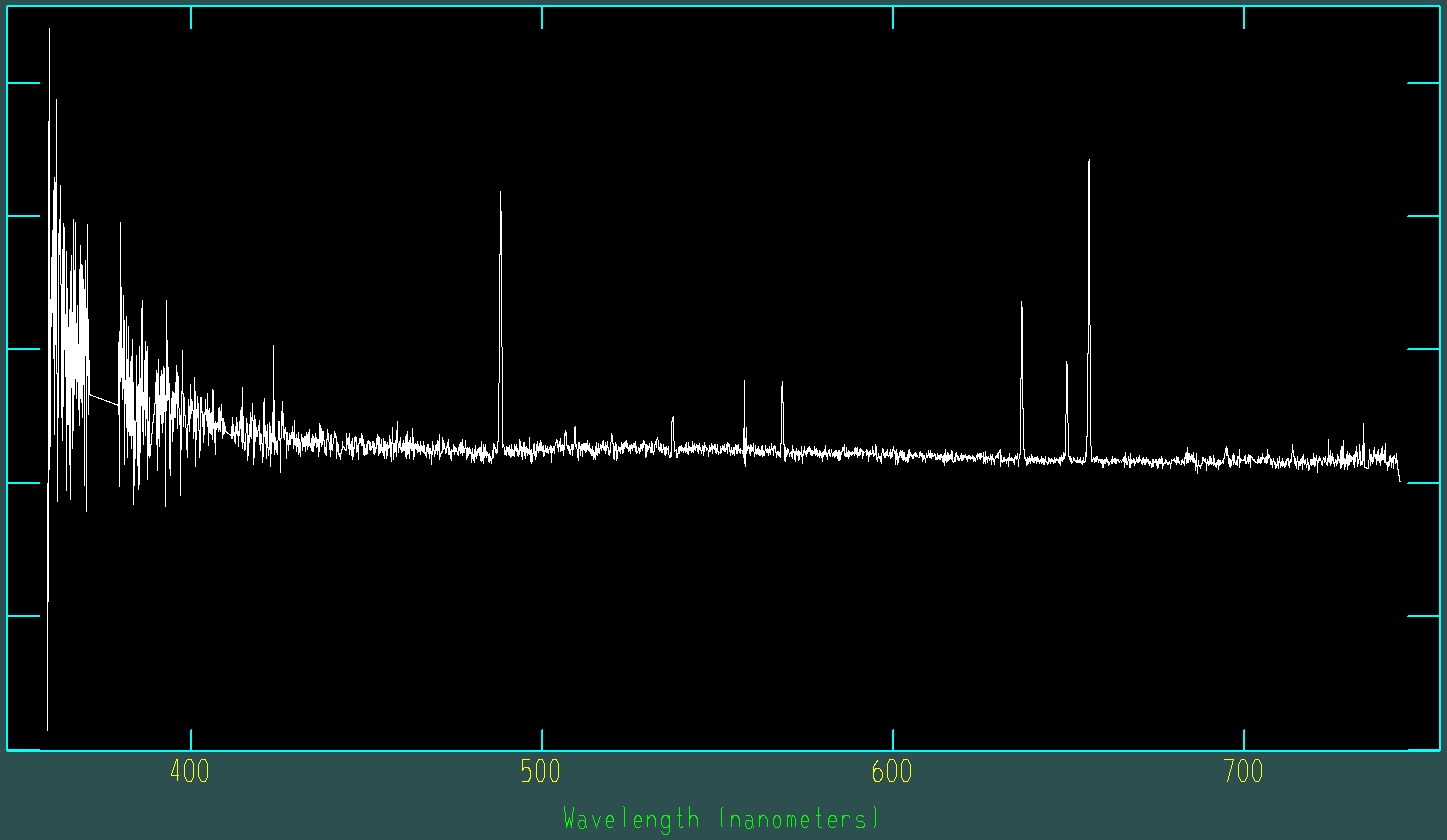
\includegraphics[width=\textwidth]{espectros/Candidate1.png}
        \caption{Candidate1}
    \end{subfigure}
    \begin{subfigure}[b]{0.45\textwidth}
        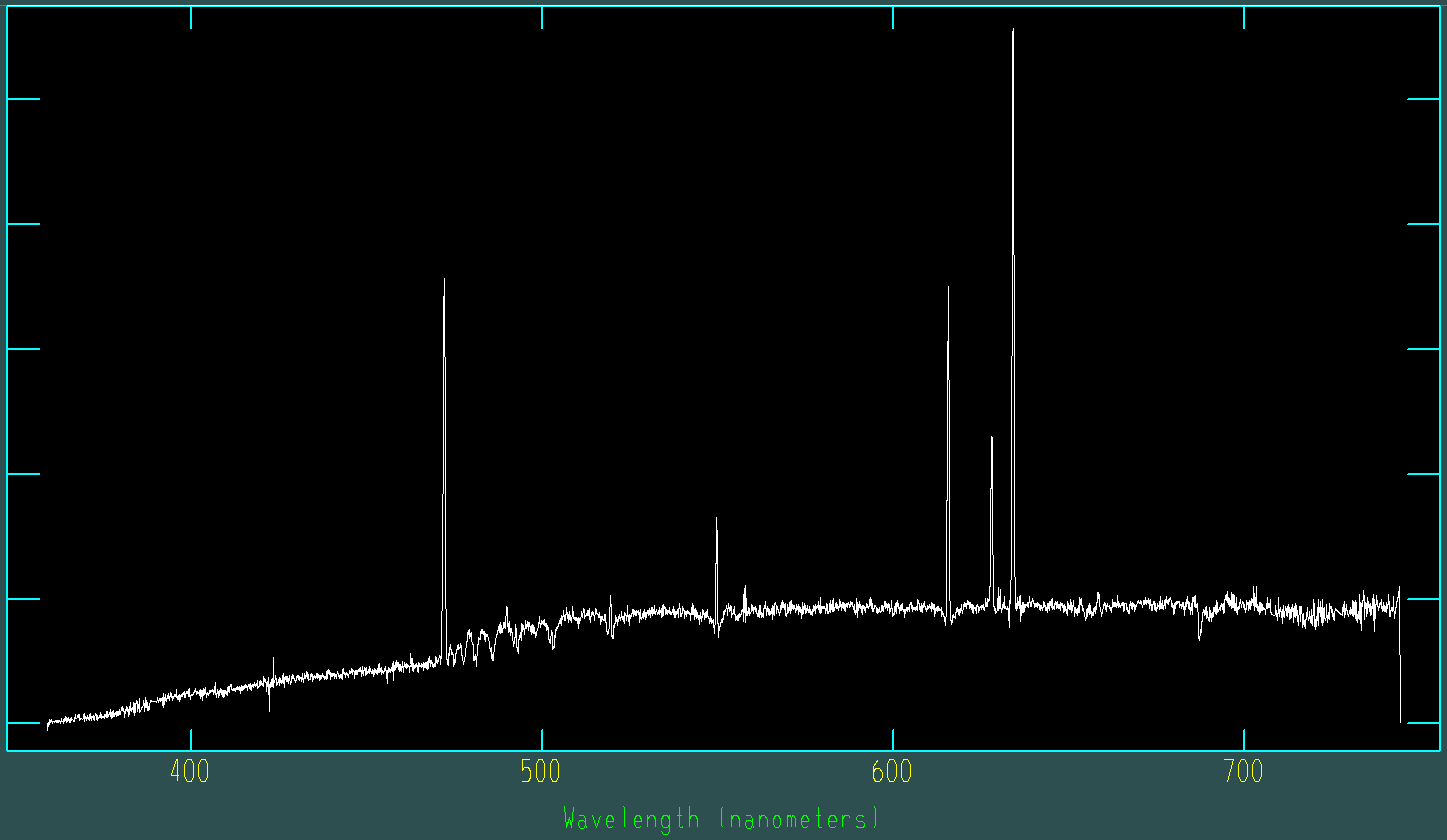
\includegraphics[width=\textwidth]{espectros/Candidate2.png}
        \caption{Candidate2}
    \end{subfigure}
    \begin{subfigure}[b]{0.45\textwidth}
        \includegraphics[width=\textwidth]{espectros/Candidate3.png}
        \caption{Candidate3}
    \end{subfigure}
    \begin{subfigure}[b]{0.45\textwidth}
        \includegraphics[width=\textwidth]{espectros/Candidate4.png}
        \caption{Candidate4}
    \end{subfigure}
    \begin{subfigure}[b]{0.45\textwidth}
        \includegraphics[width=\textwidth]{espectros/Candidate5.png}
        \caption{Candidate5}
    \end{subfigure}
    \begin{subfigure}[b]{0.45\textwidth}
        \includegraphics[width=\textwidth]{espectros/Candidate6.png}
        \caption{Candidate6}
    \end{subfigure}
    \caption{Espectros das candidatas com sinais de linhas de emissão no filtro $J0660$ observadas no Gemini Sul. Os nomes correspondem ao nome interno usado para o pedido de tempo de observação.}
    \label{espectros_candidatas_2}
\end{figure}

Analisando cada espectro e as linhas de emissão presentes, mostramos na Tabela \ref{redshift_candidatas_2} os redshifts obtidos para cada objeto, após a identificação de pelo menos duas linhas e o deslocamento em relação ao repouso.

\begin{table}[!ht]
    \centering
    \caption{Redshifts (\textit{z}) obtidos a partir dos espectros do conjunto de candidatas com sinais de linhas de emissão no filtro $J0660$ observadas com o GMOS no telescópio Gemini Sul. A coluna $OBJ_{name}$ é o nome interno da candidata utilizado no pedido de tempo do Gemini.} 
    \begin{tabular}{lcc}
        \toprule
        $OBJ_{name}$ & z   \\
        \midrule
        Candidate\_1     & 0.309 \\
        Candidate\_2     & 0.265 \\
        Candidate\_3     & 0.327 \\
        Candidate\_4     & 0.323 \\
        Candidate\_5     & 0.308 \\
        Candidate\_6     & 0.325 \\
        \bottomrule
    \end{tabular}
    \label{redshift_candidatas_2}
\end{table}

Todos os objetos mostram sinais de emissão bem definidos, especialmente onde estávamos esperando, no filtro $J0660$. Os redshifts obtidos para esses objetos estão entre 0.265 e 0.327, o que indica que esses objetos estão a uma distância considerável do aglomerado de Fornax.

Nossa ideia inicial era encontrar linhas de emissão, especificamente o $H\alpha$, que indicassem a presença de objetos compactos em Fornax, a partir apenas de uma seleção do nosso modelo com as predições. Porém, os redshifts obtidos para esses objetos indicam que eles estavam no intervalo necessário para observarmos as linhas do dupleto de $[OIII]$ no filtro $J0660$. É interessante ressaltar que, mesmo sendo objetos de fundo, eles ainda são consideravelmente compactos, e as fortes presenças de linhas de emissão indicam que podem ser galáxias com formação estelar recente, sendo um tópico interessante, mas que foge do escopo deste projeto.

Todos os objetos foram caracterizados como galáxias compactas, mostrando assim a eficiência do método de seleção de objetos compactos a partir do modelo treinado. Para a seleção desses objetos, não passamos pelos critérios com cortes nos redshifts fotométricos. Assim, mesmo não selecionando os objetos de nosso interesse, afirmamos aqui como nossa seleção foi eficiente para encontrar objetos compactos, e que a inclusão de critérios de redshifts fotométricos permite refinar ainda mais a busca.

Os resultados dos espectros desses objetos, por si só, são interessantes, visto que são objetos compactos, bem azuis, com formação estelar recente e presença de fortes linhas de emissão. Vemos na Figura \ref{redshift_candidatas_2}, para todos os objetos, a presença de diversas linhas de emissão. Na \textit{Candidate5}, por exemplo, encontramos sinais das linhas de emissão de Ne \textsc{v}, Ne \textsc{vi}, [O \textsc{ii}], He \textsc{i}, [S \textsc{ii}], H$\delta$, H$\gamma$, [O \textsc{iii}], H$\beta$, [O \textsc{iii}].

Nosso método foi capaz de recuperar galáxias compactas. Mesmo com essa pré-seleção de objetos que não estavam no aglomerado de Fornax, encontramos uma maneira de mapear e identificar objetos interessantes para estudos futuros. Em especial, concluímos que podemos encontrar objetos em redshifts por volta de 0,3, onde galáxias com fortes linhas de emissão serão evidenciadas pelo filtro estreito $J0660$.

\subsection{Seleção de candidatas com sinais de emissão} \label{subsec:candidatas_emissao}
Na subseção \ref{subsection:candidatas_emissao}, explicamos a metodologia adotada, na qual, a partir de um conjunto inicial de candidatas selecionadas com base nos cortes do modelo de separação entre objetos extensos e compactos, realizamos uma inspeção visual de vários fotoespectros para identificar aqueles que apresentavam um pico evidente no filtro $J0660$.

Os resultados do pedido de observação dessas candidatas foram obtidos e, conforme apresentado na subseção \ref{subsection:resultado_espectros_emissao}, a análise dos dados confirmou que essa estratégia foi eficaz para identificar objetos com sinais de emissão. No entanto, nenhum dos seis objetos observados foi encontrado no redshift de Fornax.

% Para as UCDs, não esperamos encontrar sinais de emissão. Assim, na primeira seleção de candidatas, adotamos apenas as probabilidades do modelo de separação entre objetos extensos e compactos, juntamente com os cortes definidos no início desta seção e os redshifts fotométricos.

Considerando que a subseleção de objetos compactos com características que evidenciam linhas de emissão sensíveis ao filtro $J0660$ se mostrou eficaz, incluímos um critério adicional que destaque esses objetos, se existirem na nossa amostra. Na Figura \ref{ex_photospec_f600}, mostramos o fotoespectro de um dos exemplos das 6 candidatas que foram observadas com sinais de emissão. Notamos como o pico no filtro $J0660$ é evidente quando o comparamos com os dois filtros adjacentes, $r$ e $i$.

\begin{figure}[!ht]
    \begin{center}
    \includegraphics[width=0.85\columnwidth,angle=0]{photo_specs/Candidate_2.png}
    \caption[]{Imagem do \textit{Photo Spec}, criada pela Ferramenta Astroinspect \cite{astroinspect}, da \textit{Candidate\_2} da lista de candidatas da subseção \ref{subsection:candidatas_emissao} de objetos compactos com sinais de linhas de emissão no filtro $J0660$.}
    \label{ex_photospec_f600}
    \end{center}
\end{figure}

Para incluir esse critério, testamos criar uma seleção em cores com esses 3 filtros que destacassem esses objetos. A cor que iremos adotar é a diferença do filtro central, $J0660$, com a média dos filtros adjacentes, $r$ e $i$. Assim, esperamos que objetos com maiores picos tenham essa cor mais destoante. A cor adotada é a seguinte:

\begin{equation}
    \text{Color\_HAlpha} = J0660 - \frac{r + i}{2}
    \label{equantion_halpha_color}
\end{equation}

Demonstrando como essa cor utilizada pode destacar essa característica, criamos um gráfico contendo parte dos objetos da nossa amostra classificados como estrela ou galáxia, comparados com os 6 objetos com sinais de emissão que encontramos anteriormente. Na Figura \ref{color_halpha}, mostramos a distribuição dessa cor para esses objetos.

\begin{figure}[!ht]
    \begin{center}
    \includegraphics[width=1.\columnwidth,angle=0]{color_halpha.png}
    \caption[]{Gráfico da cor \text{Color\_HAlpha} em função da magnitude \textit{r\_APER\_6}. Pontos em azul são todos os dados da amostra de Fornax. Pontos em verde e vermelho são os objetos classificados como galáxias ou estrelas pelo GAIA DR3, respectivamente. Estrelas em amarelo são os 6 objetos com sinais de emissão que foram observados.}
    \label{color_halpha}
    \end{center}
\end{figure}

Pela Figura \ref{color_halpha}, notamos que os objetos com sinais de emissão se destacam a partir de um corte em \text{Color\_HAlpha}$\leq$-0.2. Vale ressaltar que, devido aos erros nos filtros e às diferenças entre as bandas $r$, $i$ e $J0660$, não necessariamente objetos com essa cor abaixo desse valor são representativos de terem um pico em $J0660$. Existem casos onde essa cor pode ser intensa devido a uma diferença brusca, de uma grande subida ou descida entre o filtro $i$ e $J0660$ ou $r$ e $J0660$, e não um pico propriamente dito. Então, mesmo sendo capaz de filtrar esses objetos, ainda precisamos avaliar visualmente os fotoespectros.

Da amostra de candidatas final selecionadas na seção \ref{cap:selecao_candidatas}, aplicamos um corte de \text{Color\_HAlpha}$\leq$-0.3, para identificar objetos com sinais de emissão. Obtivemos 49 objetos com essa cor abaixo do corte. Mostramos na Figura \ref{halpha_candidatas_final} o fotoespectro de exemplo desses 4 objetos.

\begin{figure}[!ht]
    \centering
    \captionsetup{justification=centering}
    \begin{subfigure}[b]{0.45\textwidth}
        \includegraphics[width=\textwidth]{photo_specs/candidate_final/candidate_final_1.png}
        \caption{a)}
    \end{subfigure}
    \begin{subfigure}[b]{0.45\textwidth}
        \includegraphics[width=\textwidth]{photo_specs/candidate_final/candidate_final_2.png}
        \caption{b)}
    \end{subfigure}
    \begin{subfigure}[b]{0.45\textwidth}
        \includegraphics[width=\textwidth]{photo_specs/candidate_final/candidate_final_3.png}
        \caption{c)}
    \end{subfigure}
    \begin{subfigure}[b]{0.45\textwidth}
        \includegraphics[width=\textwidth]{photo_specs/candidate_final/candidate_final_4.png}
        \caption{d)}
    \end{subfigure}
    \caption{Imagens dos \textit{Photo Spec}, criadas pela Ferramenta Astroinspect \cite{astroinspect}, com corte na cor criada pela equação \ref{equantion_halpha_color}, aplicando um corte abaixo de -0.3 na lista de candidatas finais a objetos compactos de Fornax da seção \ref{cap:selecao_candidatas}.}
    \label{halpha_candidatas_final}
\end{figure}

Concluímos que a metodologia de seleção de objetos compactos foi eficaz em identificar objetos com características interessantes, mesmo em intervalos de redshift em torno de 0.3, ainda que não sejam UCDs. Esses objetos podem ser explorados em projetos futuros, especialmente devido à presença de fortes linhas de emissão, que indicam formação estelar ativa.

Além disso, ao final do processo, identificamos uma lista de quatro objetos que podem ser relevantes para estudos futuros de galáxias compactas com linhas de emissão, selecionados com base em cortes de redshift fotométrico para o aglomerado de Fornax. Embora esses objetos não sejam UCDs, sua natureza compacta e os sinais de emissão observados os tornam candidatos promissores para investigações adicionais, ampliando o escopo de estudos sobre a diversidade de objetos compactos no universo.


